\documentclass[10pt,twocolumn,letterpaper]{article}

\usepackage{cvpr}
\usepackage{times}
\usepackage{epsfig}
\usepackage{graphicx}
\usepackage{amsmath}
\usepackage{amssymb}
\usepackage{csvsimple}
\usepackage{subcaption}
% for \FloatBarrier to keep figs in sections
\usepackage[section]{placeins}

% color text
\usepackage{color}

\newcommand{\todo}[1]{\textcolor{red}{#1}}

% Include other packages here, before hyperref.

% If you comment hyperref and then uncomment it, you should delete
% egpaper.aux before re-running latex.  (Or just hit 'q' on the first latex
% run, let it finish, and you should be clear).
\usepackage[breaklinks=true,bookmarks=false]{hyperref}

\cvprfinalcopy % *** Uncomment this line for the final submission

\def\cvprPaperID{****} % *** Enter the CVPR Paper ID here
\def\httilde{\mbox{\tt\raisebox{-.5ex}{\symbol{126}}}}

% Pages are numbered in submission mode, and unnumbered in camera-ready
%\ifcvprfinal\pagestyle{empty}\fi
\setcounter{page}{1}
\begin{document}

%%%%%%%%% TITLE
\title{Understanding the Amazon from Space}

\author{Vishal Subbiah*\\
Stanford University\\
{\tt\small svishal@stanford.edu}
% For a paper whose authors are all at the same institution,
% omit the following lines up until the closing ``}''.
% Additional authors and addresses can be added with ``\and'',
% just like the second author.
% To save space, use either the email address or home page, not both
\and
Brent Lunghino*\\
Stanford University\\
{\tt\small lunghino@stanford.edu}
\and
Brian Rohr*\\
Stanford University\\
{\tt\small brohr@stanford.edu}
}



\maketitle
%\thispagestyle{empty}

%%%%%%%%% ABSTRACT
\begin{abstract}
   In this work, we use convolutional neural networks to assign atmospheric conditions labels and land usage labels to satellite images of the Amazon Rainforest. Convolutional Neural Networks have successfully been used previously on various satellite imagery classification. We have trained several neural networks including custom convolutional architectures, ResNets and GoogleNets. Our best result is 0.918 (F2 score) on the test set.
\end{abstract}

\footnotetext{*All authors contributed equally to this work.}

%%%%%%%%% BODY TEXT]

\section{Introduction}

	The Amazon Rainforest is extremely important to preserve due to its unmatched biodiversity and great capacity to uptake carbon dioxide \cite{WWF}, but it is difficult to make a case for the urgency of its preservation without first quantifying the rate of its destruction.  Since the Amazon covers a 5.5 million square kilometer area, understanding and quantifying the changes in land use there over the years is a formidable task. With a great deal of effort, humans could classify one set of satellite images of the Amazon, but it is intractable for humans to go through satellite images of the entire rainforest one by one and manually label how the land is being used, and this task would need to be completed many times in order to understand how the land use is changing over time.

For that reason, we have trained deep convolutional neural networks that will be able to rapidly process satellite images of the Amazon and output labels and metrics that quantify how the land is being used. Specifically, the model takes satellite images of the Amazon rain forest as inputs and outputs one or many of seventeen possible labels for each image. This model will be able to be used to classify the remaining hundreds of thousands of images that are not in the training set, and it will be able to be used to classify new images that are taken at future time points. With this machine learning image processing technique, temporal land use data will be easily assembled, providing the necessary data to make a case for protecting the Amazon Rainforest. Furthermore, satellite data of the rain forest can be applied to compute deforestation rates, detect illegal mining/deforestation, and differentiate between natural and human-caused deforestation.


%------------------------------------------------------------------------
\section{Related Work}

Many previous studies have applied convolutional neural networks to a variety of machine learning problems that use satellite images and other remote sensing data as inputs with some success. Models that predict a single label for each satellite image have achieved a test accuracy of greater than 99\%. \cite{background4}. Convolutional neural networks have also been used successfully on satellite image segmentation problems. \cite{background3} \cite{segmentation1}
The key advantage of using convolutional neural networks as opposed to other machine learning techniques is that convolutional neural networks are able to learn problem-specific features of the input images that help with the classification or segmentation problem at hand. \cite{background2} This has been shown to be true for many applications in remote sensing image labeling from crop identification to poverty mapping. \cite{background1} \cite{Ensemble1} \cite{PovertyMapping}

Previous studies have used a variety of convolutional neural net architectures. These architectures include standard convolutional architectures, similar to VGG-Net\cite{VGGNet} as well as newer architectures, similar to ResNet\cite{ResNet} and GoogleNet\cite{GoogleNet}. In general, in studies applying these techniques to satellite image classification, the newer architectures give better accuracies than the VGG-Net-like architectures.\cite{VGG1} \cite{Inception1} \cite{TransferLearning3} \cite{TransferLearning1}

Previous studies have also employed a variety of training techniques. In this field, it is popular to use transfer learning: to begin with a convolutional neural net that has already been trained on ImageNet,\cite{imagenet} and then fine-tune the network for the new application. Several studies report good results using transfer learning for satellite image classification problems. \cite{TransferLearning2} \cite{TransferLearning3} \cite{TransferLearning5} \cite{TransferLearning1} \cite{TransferLearning4} However, some studies report that for particular architectures, training from scratch gives better results than fine-tuning a pre-trained network.\cite{fromscratch2} Additionally, previous work has reported that using data augmentation and ensembling improves the accuracy on the test set. \cite{TransferLearning4} \cite{Ensemble1} Furthermore, importantly, it has been shown that models trained on satellite images of one region can be successfully applied to unseen regions.\cite{PovertyMapping} For example, a neural network trained on images of one set of cities was able to perform well on completely unseen cities. \cite{TransferLearning5} Overall, it has been shown that convolutional neural networks are very useful for automatic satellite image labeling tasks.


%------------------------------------------------------------------------

\section{Methods}
Our goal is to train a neural network that gives a high F2 score on the validation set. We have implemented many architectures and used cross-validation to tune hyperparameters and select the best architecture. We implement the methods discussed below using PyTorch \cite{PyTorch} and scikit-learn \cite{scikit-learn} \footnote{We used CS 231N assignment 2 code as a starter for our project}.

The $F_{\beta}$ score is defined as:
\begin{equation} \label{eq:F2_score}
F_{\beta} = (1+\beta^2) \frac{p \cdot r}{\beta^2p + r}
\end{equation}

Where precision is the ratio of true positives to all predicted positives defined as $p = \frac{tp}{fp + tp}$ and recall is the ratio of true positives to predicted positives and incorrectly predicted negatives defined as $r = \frac{tp}{tp + fn}$.

\subsection*{Enhancing training speed} To enhance training speed, we will use the Adam optimizer\cite{Adam}, which generally finds local minima in lesser iterations than stochastic gradient descent. Our optimizer has an adaptive learning rate that scales down when loss decay stagnates \cite{Liu2017}. We performed our initial hyperparameter tuning on a subset of the training data set in order to quickly identify a good order of magnitude for each hyperparameter. Also, since the learning rate, one of the most important hyperparameters, decays automatically, it is sufficient to set the learning rate to any reasonable number. Then, the algorithm will attenuate the learning rate over time, allowing the loss to settle to the bottom of the minimum in the high-dimensional loss landscape.

\subsection*{Activation Functions}
In this work, the activation function is the rectified linear activation unit (ReLU), which has many advantages and some disadvantages. The principal advantage is that it is very simple and computationally efficient, and it provides the necessary non-linearity that allows the model to capture more complex relationships within the data. One downside of the ReLU activation function is that it has zero slope over half of its domain. Therefore, during backpropagation, it can pass zero derivatives backwards, causing all parameters directly downstream from that activation function to receive no information about the gradient of the loss upstream from that activation function.

\subsection*{Overfitting/Underfitting (Bias/Variance Analysis)} It is important to keep track of whether the model is overfit or underfit. To check how overfit or underfit our model is, we will monitor the loss, validation accuracy, and training accuracy as a function of epoch for each set of hyperparameters that we use. If the validation accuracy begins to suffer while the training accuracy continues to increase, we know that our model has overfit. However, if the loss converges quickly and the training accuracy and validation accuracy are similar, we will know that the model is underfit. Some methods that we can use to fight against overfitting or underfitting are regularization, data augmentation, and model complexity. If the model is overfit, we could increase regularization strength, decrease the model's complexity, or add data augmentation. If the model is underfit, we could decrease regularization or increase the model's complexity by adding more layers or more filters in the convolutional layers.

\subsection*{Sigmoid Cutoff Optimization} Each of our models outputs a score for each label representing how strongly the model believes that label should be assigned to the input image. The scores are then passed through a sigmoid function so that they are between zero and one. Labels are independently assigned a True (the label should be assigned to the image) or False (the label should not be assigned to the image) depending whether the sigmoid of the score for that class is above a certain cutoff. After training a model and outputting the sigmoid of the scores, we run a brute force optimization on the values of these cutoffs for each class to maximize the F2 score on the validation set.

\subsection*{Ensemble Weights Optimization} Some of our architectures involve training multiple convolutional neural networks in parallel and combining the results with a weighted sum. For these architectures, we express the F2 score as a function of the weights and determine the optimal weights by using Particle Swarm Optimization \cite{kennedy2011particle} maximize the F2 score.

\subsection*{Batch Balancing} Some labels are very common and others are very rare. To ensure that our model learns about the rare labels as well as the common ones, we have implemented batch balancing functionality. This functionality, when turned on, ensures that the model sees all labels equally frequently despite the fact that the training set is very unbalanced.

\subsection*{Architectures:}
\subsection*{6-layer CNN}

The first deep convolutional neural net presented in this work is a 6 layer net built from scratch. The model takes in the 256 x 256 x 4 images and passes them through a convolution layer with 16 filters with size 3x3, stride 1, and pad 1. We use a ReLU activation function on the result followed by a batch normalization layer. After that, a max pooling layer is applied with kernel size 2, stride 2, pad 0. This conv - ReLU - batch normalization - max pool block is applied 6 times, and the result is flattened and passed through two fully connected layers with 1024 hidden nodes and 17 outputs, respectively.

This network design takes capitalizes on the core principle of convolutional layers: During training, the filters are modified to look for the for the features most relevant to our labeling task. However, this design does not benefit from any of the advantages of the more recently developed architectures. These advantages are described in the subsequent sections.

\subsection*{GoogleNet}
This model takes in 256x256x3 RGB images as the input. The first layer is a convolutional layer with 32 filters of kernel size 3, stride 1, pad 1 so the output image height and width is the same as the input image. Next, the model has two inception modules, inspired by GoogleNet.\cite{GoogleNet} Each inception module has 16 1x1 filters, 16 3x3 filters, and 16 5x5 filters. The output of the inception modules is flattened and passed through a final affine layer, giving scores the scores for each of the 17 classes.

This model uses convolutional layers of different kernel sizes, and the output is concatenated. The advantage of this approach is that the model is able to look for features of different sizes. One downside is that the model is much slower to train.

\subsection*{ResNets}
This model takes in 224x224x3 RGB images as the input. The first layer is a standard convolutional layer with 64 filters with kernel size 7, stride 1, pad 3, so the output image height and width is maintained and now has depth 64. The next layer is a max pooling layer with kernel size 2, stride 2, pad 0, so the output image is half the height and half the width of the input image. Next, there are any number of "residual blocks." A residual block takes the input and passes it through 2 convolutional layers (with a ReLU activation layer in between them) with 64 filters with kernel size 3x3, stride 1, pad 1, so the output size is the same as the input size. The distinguishing feature of this architecture is that the output of these convolutional layers is added to the input, and this sum is passed on to the next layer. In this work, we present models with 18, 50, 101 residual blocks. Finally, the output is passed through an average pooling layer and an affine layer to yield the scores for the 17 classes.

This architecture has many advantages. Most importantly, during backpropagation, the derivative of the loss function is passed directly to each residual block. This helps greatly to prevent very deep architectures from suffering from vanishing gradients. Furthermore, the pair of 3x3 convolutional layers in each residual block has the same receptive field as a single 5x5 convolutional layer, but it requires fewer parameters. Also, due to the ReLU activation function between the two convolutional layers in each residual block, the block is able to identify more non-linearities than the single 5x5 filter.

This model gives our best results, and it is the one that has been used for the majority of our experimentation. A diagram of a ResNet-34 is included above.

\begin{figure}
    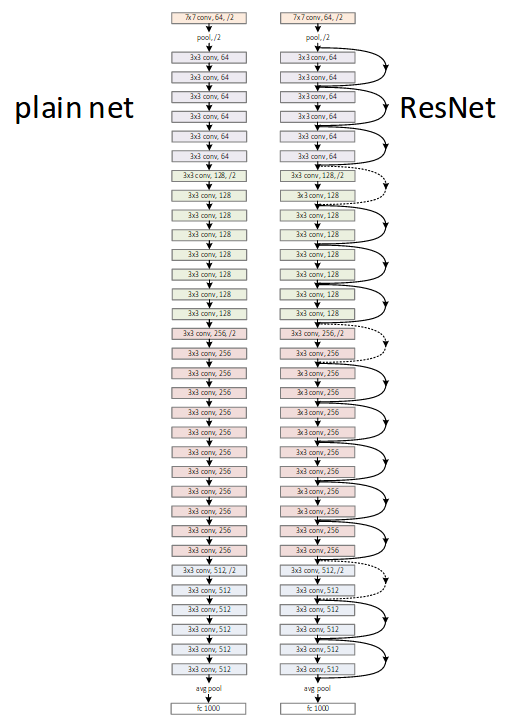
\includegraphics[width=\columnwidth]{fig/resnet_vs_plainnet.png}
    \caption{Schematic of ResNet architecture compared to traditional neural network \cite{ResNet}}
    \label{fig:resnet_plainent}
\end{figure}



\begin{figure}
\begin{subfigure}{.5\columnwidth}
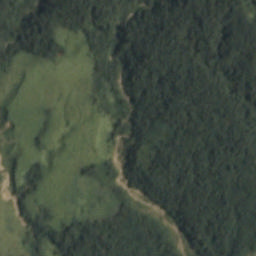
\includegraphics[width=0.9\columnwidth]{sample_images/train_1.jpg}
\caption{jpg of Sample 1}
\end{subfigure}%
\begin{subfigure}{.5\columnwidth}
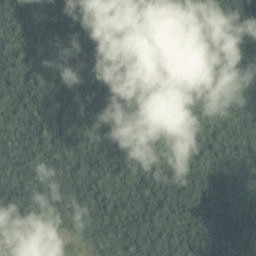
\includegraphics[width=0.9\columnwidth]{sample_images/train_1000.jpg}
\caption{jpg of Sample 2}
\end{subfigure}
\begin{subfigure}{.5\columnwidth}
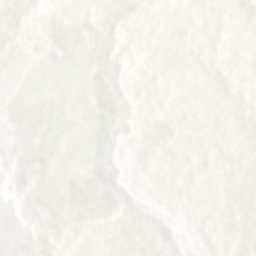
\includegraphics[width=0.9\columnwidth]{sample_images/train_1_tif.png}
\caption{tif of Sample 1 with infrared}
\end{subfigure}%
\begin{subfigure}{.5\columnwidth}
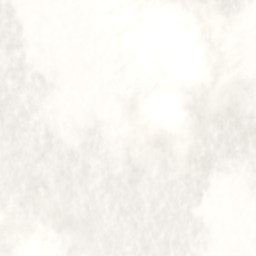
\includegraphics[width=0.9\columnwidth]{sample_images/train_1000_tif.png}
\caption{tif of Sample 2 with infrared}
\end{subfigure}
\begin{subfigure}{.5\columnwidth}
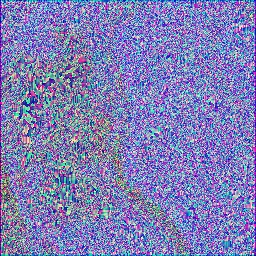
\includegraphics[width=0.9\columnwidth]{sample_images/train_1_grad.jpg}
\caption{gradient image of Sample 1}
\end{subfigure}%
\begin{subfigure}{.5\columnwidth}
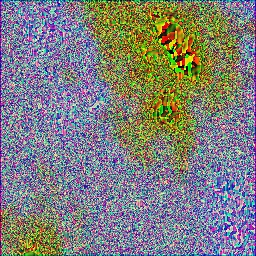
\includegraphics[width=0.9\columnwidth]{sample_images/train_1000_grad.jpg}
\caption{gradient image of Sample 2}
\end{subfigure}
\begin{subfigure}{.5\columnwidth}
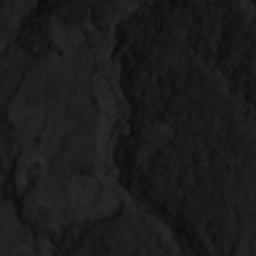
\includegraphics[width=0.9\columnwidth]{sample_images/train_1_inf.png}
\caption{Infrared image of Sample 1}
\end{subfigure}%
\begin{subfigure}{.5\columnwidth}
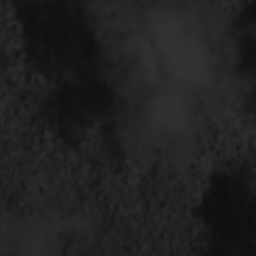
\includegraphics[width=0.9\columnwidth]{sample_images/train_1000_inf.png}
\caption{Infrared image of Sample 2}
\end{subfigure}
\caption{Sample 1 is classified as agriculture, clear, primary and water while Sample 2 is classified as partly cloudy and primary}
\label{fig:exp_images}
\end{figure}
%------------------------------------------------------------------------
\section{Problem Statement, Data Set, and Features}
\subsection*{Data Set Details}
The goal is to train a model that can take a satellite image of the Amazon Rainforest as the input and output a 1 or a 0 for each of 17 possible labels. The labels are cloudy, partly cloudy, hazy, primary rainforest, water, habitation, agriculture, road, cultivation, bare ground, slash and burn, selective lodging, blooming, conventional mining, artisinal mining, and blow down. Each image could one or many labels. For example, an image may have roads, water, habitation, and primary rainforest, and another image could have just primary rainforest. The only constraint is that each image must have at least one label. The data is provided by Planet for a Kaggle competition\cite{Kaggle}. The training data set is 40,000 images with an additional 60,000 image test set. During each training epoch, 10\% of the training data was used for validation, and the validation set is chosen at random. Each image is 256x256 pixels with 4 bands of color (RGB + near-infrared). Each image captures a land area of 947 meters x 947 meters, giving a resolution of 3.7 meters per pixel. The dataset covers 30 million hectares of Amazon Rainforest. Each of the 40,000 training examples has already been manually labeled as either having or not having each of the 17 possible labels.

The class distribution among the labels is not at all balanced. For example, the labels "primary forest" and "clear" (weather) each appear in more than 25,000 of the 40,000 training images, while "conventional mine" and "blow-down" appear extremely infrequently \cite{KaggleKernel}.

\begin{figure}
    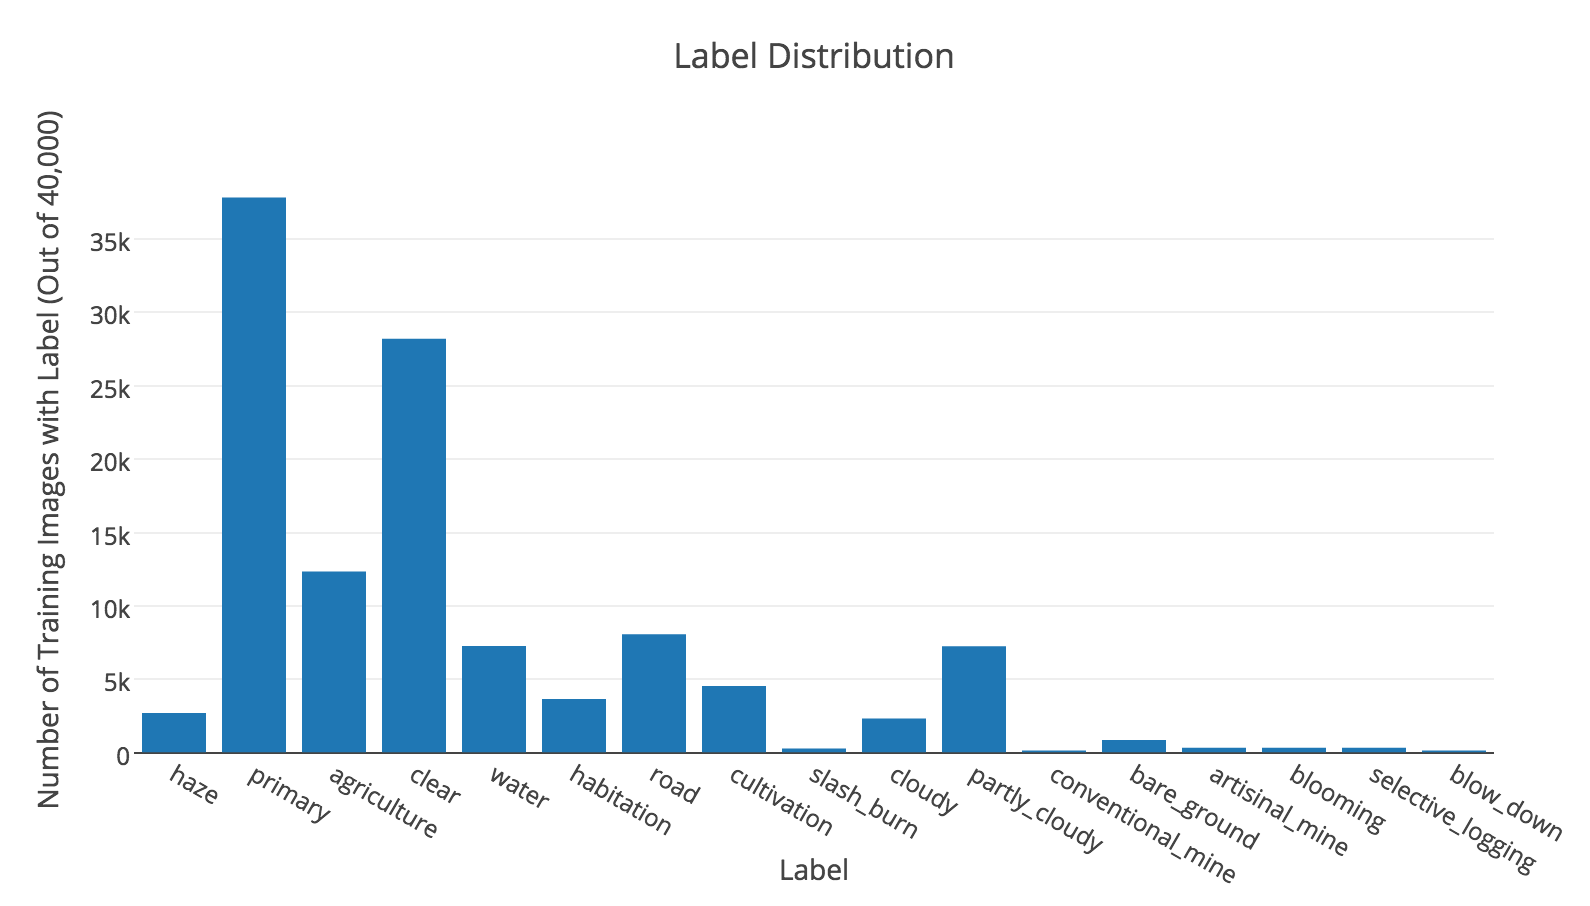
\includegraphics[width=\columnwidth]{fig/Screen_Shot_2017-06-12_at_8_10_06_PM.png}
    \caption{Label Distribution \cite{KaggleKernel}}
    \label{fig:labeldist}
\end{figure}

\subsection*{Preprocessing}
Some of the models presented were pretrained on ImageNet.\cite{imagenet} In these cases, the images are normalized based on the mean and standard deviation of the images in the ImageNet dataset. When training models from scratch, the images were normalized according to the mean and standard deviation of the entire training set (per channel).

For some models, additional preprocessing steps are taken. The original data consists of 3 channel RGB data from atmospherically corrected .jpg images and 4 channel RGB + near-infrared (NIR) data from uncorrected radiance stored as .tif files. These can be seen in Figure \ref{fig:exp_images} a - d. Other unique color channels were constructed from this data. We mapped the NIR channel to 3 color bands, shown in \ref{fig:exp_images} g-h. We also generated the gradients along X and Y for the gray scale image, shown in \ref{fig:exp_images} e - f. The gradient images may look noisy at first glance, but they actually contain unique information. For example, the cloud can be easily seen in the top right of figure f. After training separate networks in parallel on data sets that had been pre-processed differently then combining the results, we actually achieved a higher F2 score on the F2 set than any of the individual models.

\subsection*{Data Augmentation}
Data augmentation is a crucial strategy for fighting overfitting. When training the models presented, the input images were randomly rotated and flipped then randomly cropped from 256x256 to 224x224. Using these two methods of data augmentation, the model likely never sees the exact same training example twice during training.  
%------------------------------------------------------------------------

\section{Experiments, Results, and Discussion}

We have explored a variety of models to maximize our F2 score accuracy.  A summary of the results for our models is presented in Table \ref{tab:summary}. The best model is the triple ResNet18 which achieved an F2 score of 0.918 on the test dataset. Figure \ref{fig:correct_labels} shows examples of images for which our best model assigned all correct labels, partially correct labels, and completely incorrect labels. The model successfully classifies common labels, such as primary forest and clear skies but struggles to classify less common labels, such as agriculture. The model also struggles to predict features that only occupy a small portion of the image. Each model that we developed is described below along with an assessment of its performance and its contribution to the development process.

\begin{figure}[h]
\begin{subfigure}{0.5\columnwidth}
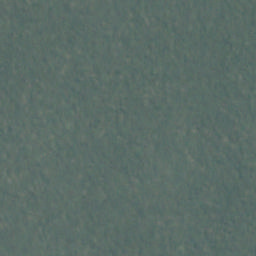
\includegraphics[width=0.9\columnwidth]{sample_images/train_0.jpg}
\caption{Correct: clear, primary;\\Predicted:clear, primary }
\label{subfig:all}
\end{subfigure}%
\begin{subfigure}{0.5\columnwidth}
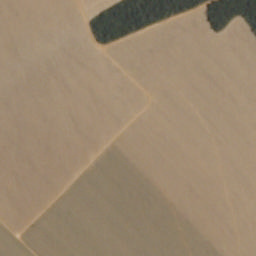
\includegraphics[width=0.9\columnwidth]{sample_images/train_122.jpg}
\caption{Correct:agriculture, haze, primary, water; Predicted:cloudy }
\label{subfig:none}
\end{subfigure}
\begin{subfigure}{\columnwidth}
\centering
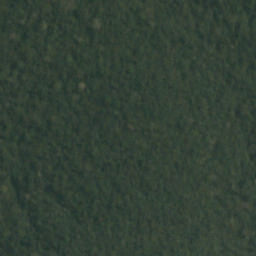
\includegraphics[width=0.45\columnwidth]{sample_images/train_3.jpg}
\caption{Correct: agriculture, cultivation, partly cloudy, primary\\Predicted:agriculture, clear, cultivation, primary, road}
\label{subfig:some}
\end{subfigure}
\caption{Qualitative results: example images for which the model assigned all labels correctly \ref{subfig:all}, no labels correctly \ref{subfig:none}, and some labels correctly \ref{subfig:some}}
\label{fig:correct_labels}
\end{figure}

\begin{table}
  \centering
  \begin{tabular}{|l|c|c|}
  \hline
  \csvreader[column count=3,
    no head,
    table head=\hline,
    late after line=\\,  
    late after first line=\\\hline
  ]{231N_models.csv}{}
  {\csvcoli & \csvcolii & \csvcoliii}
  \hline
  \end{tabular}
  \caption{Summary of trained models and results}
  \label{tab:summary}
\end{table}

\subsection*{6-layer CNN}
This was a simple architecture that was implemented first as a baseline from which to build on. After training for 10 epochs, the validation accuracy plateaus at 0.83, as seen in Figure \ref{fig:acc_6_layer}. Since, at the end of 10 epochs of training, the training accuracy is still increasing, but the validation accuracy has plateaued, this model is beginning to overfit the training data, and further training would likely not result an increase in F2 score on the validation or test set. Since other network architectures, like GoogleNet and Resnet, have performed better in the ImageNet competition,\cite{imagenet} we quickly moved on to these state-of-the-art architectures.

\begin{figure}
    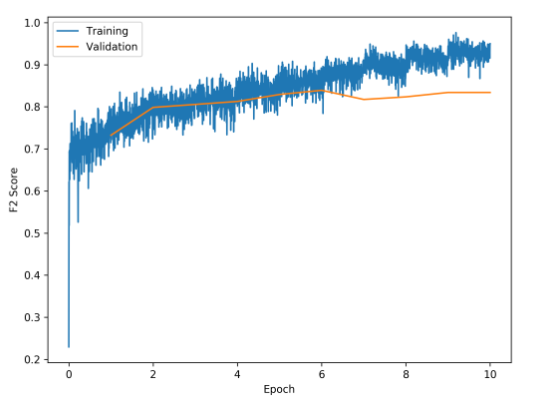
\includegraphics[width=\columnwidth]{fig/AccuracyCurve.png}
    \caption{Accuracy (F2 score) for the training set and the validation set as a function of epoch. The training accuracy was plotted at the end of each batch of data, and the validation accuracy was plotted at the end of each epoch.}
    \label{fig:acc_6_layer}
\end{figure}

\begin{figure}
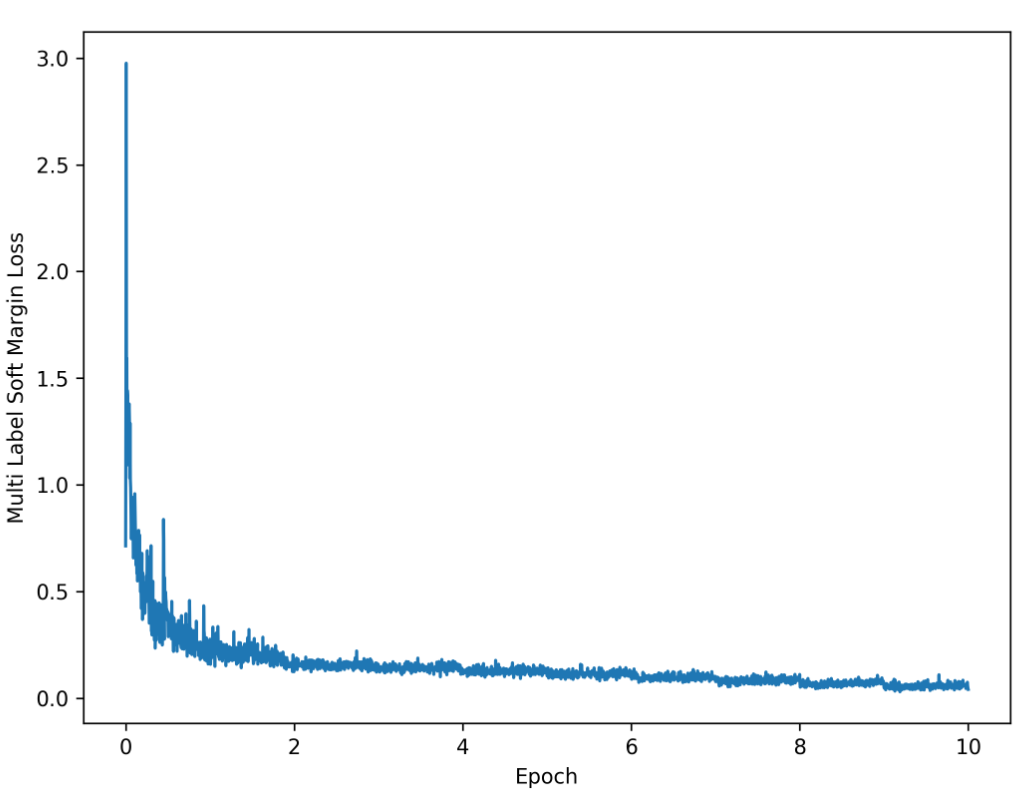
\includegraphics[width=\columnwidth]{fig/LossCurve.png}
    \caption{Training loss (PyTorch multilabel soft margin loss) as a function of epoch. It is clear that learning rate decay was introduced near the start of the second epoch, and after 10 epochs the loss is approximately converged.}
\end{figure}

\subsection*{GoogleNet}

The GoogleNet architecture outperformed the simple 6-layer CNN with an F2 score of 0.86 on the validation set. This model took much longer to train, however. Since the training and validation accuracy for this model were nearly identical, it is likely that the model is underfit, and a more complex model would give better results. It would be a reasonable next step to try to train a GoogleNet with more inception modules or more filters in each inception module or additional affine-ReLU layers at the end, however, this option was not pursued. Instead, we explored the ResNet architecture in more depth because the time required to train an epoch was much lower in the ResNet case, and the ResNet architecture performed slightly better in previous image classification tasks. \cite{TransferLearning1} \cite{imagenet}

\subsection*{Pretrained ResNet18}

One strategy we explored was fine-tuning pretrained models \footnote{Pretrained model code was based off the example of \cite{Johnson2017}}. Our first effort with this strategy was to fine-tune a ResNet18 initialized with weights from training on the Imagenet dataset. Before fine-tuning, we resized the final fully connected layer to output 17 scores instead of the 1000 used for Imagenet classification. The final fully connected layer was trained individually for 4 epochs at a high learning rate (1e-3). After the loss had stopped decreasing by training only the final fully connected layer, (Figure \ref{fig:plot_loss_resnet18_pretrained_fc}) we dropped the learning rate (to 1e-5) and began updating the weights for all layers of the model. In this fine-tuning stage, the loss is able to decrease further (Figure \ref{fig:plot_loss_resnet18_pretrained_tune}). The batch size was 256 images per batch. This model performed quite well considering how quickly it trained and how simple the model was. The F2 score for this model on the validation set was 0.887, which is only about 0.04 less than that of our top-performing models. Since the training and validation accuracy were very similar for this model, it is likely that the model is underfit, and the quantity of data we have warrants a more complex, deeper model.

\begin{figure}
	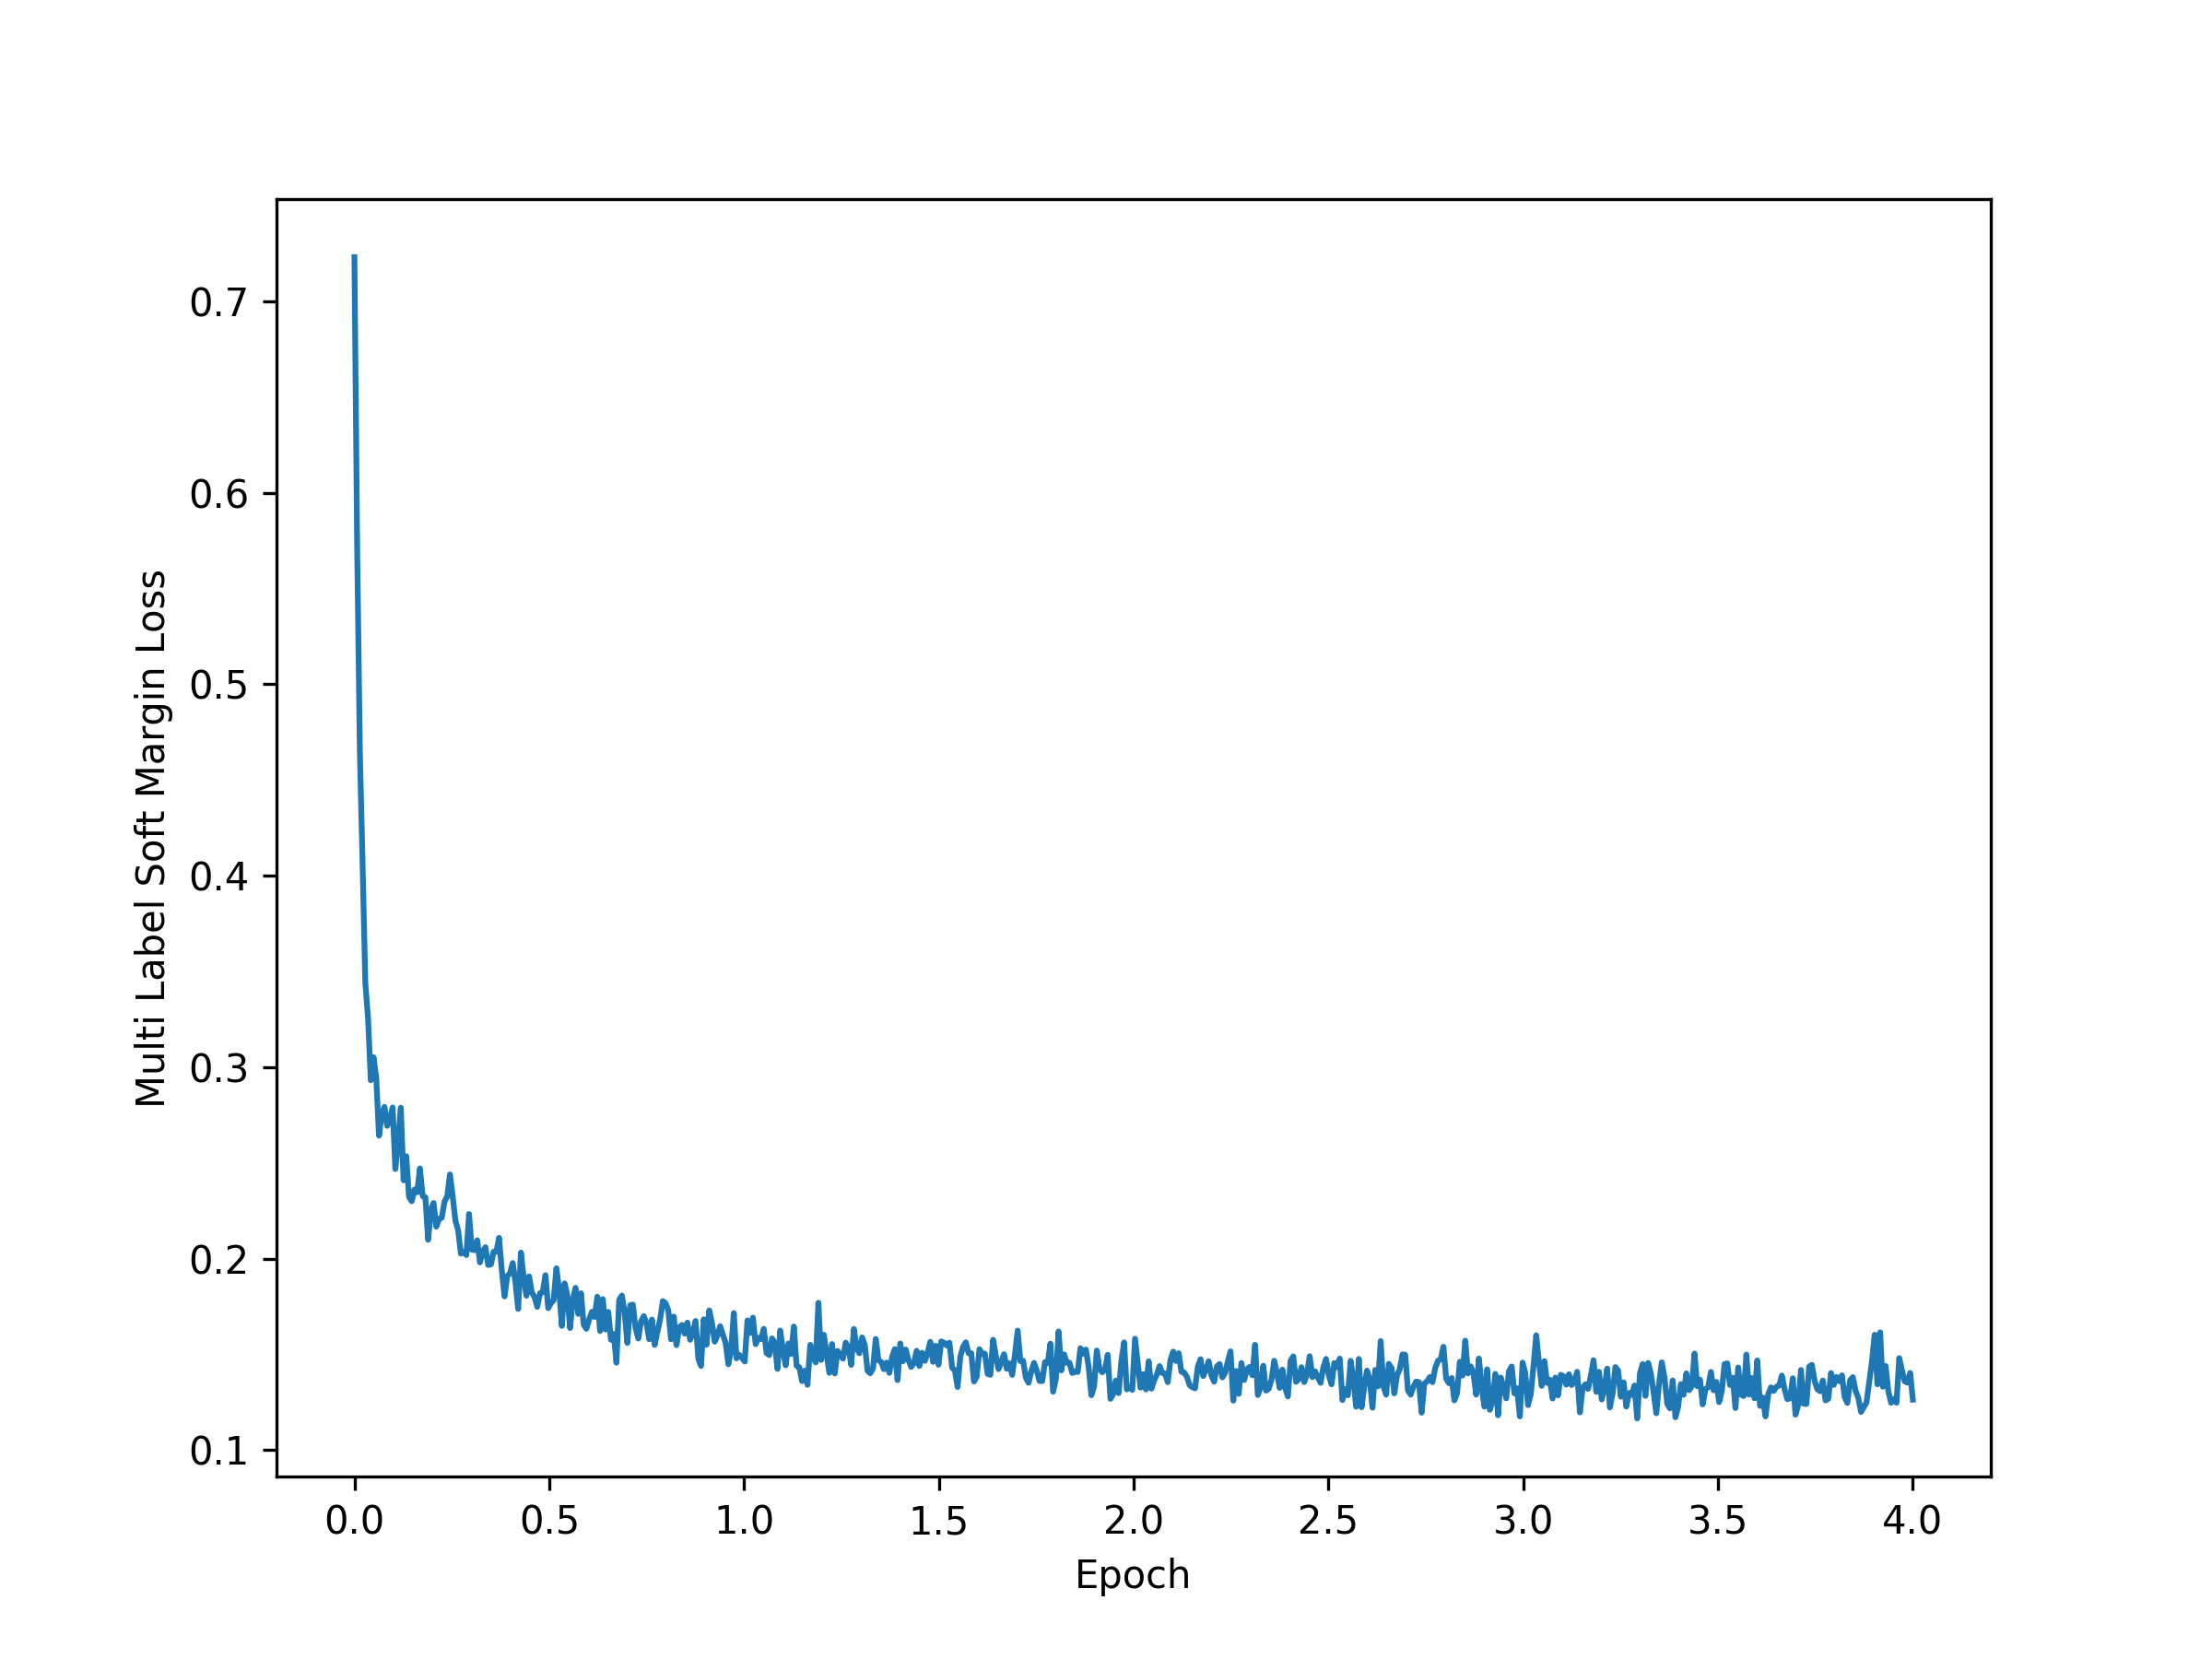
\includegraphics[width=\columnwidth]{fig/plot_loss_resnet18_pretrained_fc.png}
    \caption{Pretrained ResNet18, loss during training of final fully connected layer}
    \label{fig:plot_loss_resnet18_pretrained_fc}
\end{figure}

\begin{figure}
	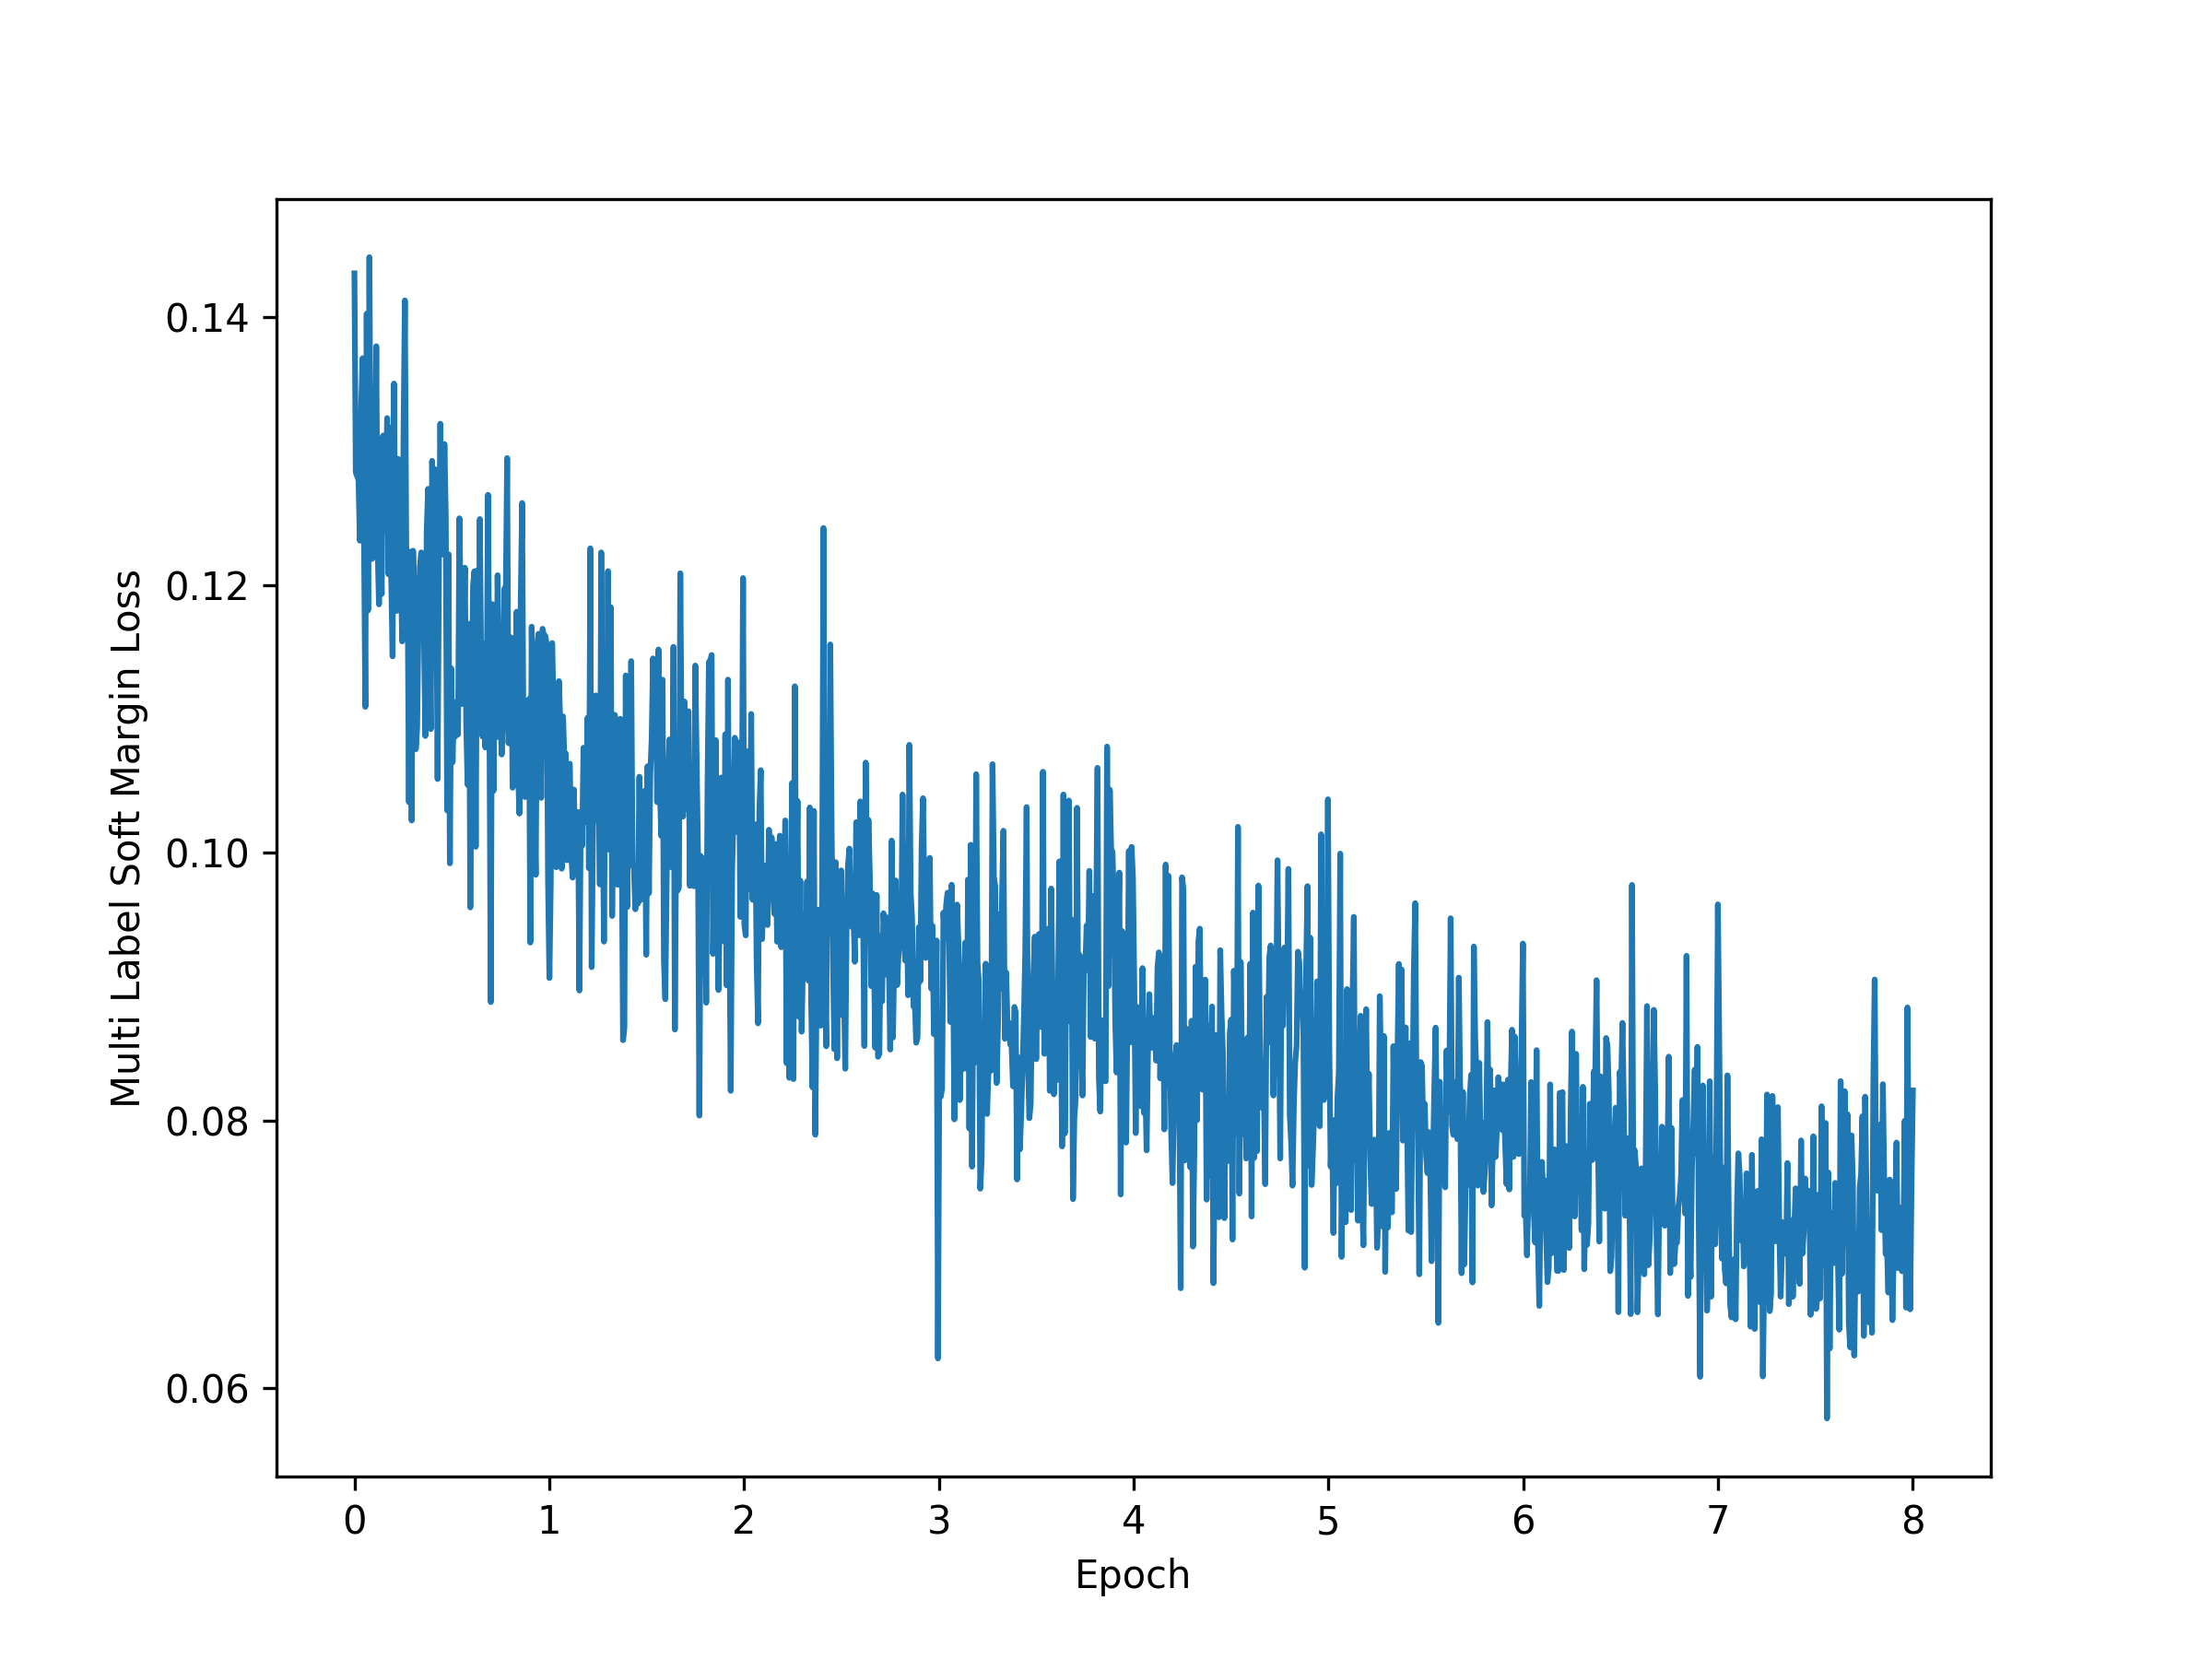
\includegraphics[width=\columnwidth]{fig/plot_loss_resnet18_pretrained_tune.png}
    \caption{Pretrained ResNet18, loss during fine-tuning of all model weights}
    \label{fig:plot_loss_resnet18_pretrained_tune}
\end{figure}

\subsection*{Pretrained ResNet101}

Our next strategy was to pursue the same approach described above, but applied to a deeper model: ResNet101. We fine-tuned a pretrained ResNet101 using the same training hyperparameters developed for ResNet18 but with a smaller batch size of 32 instead of 256. The reason for the smaller batch size was simply to decrease memory usage: the deeper model has many more parameters per image, so it can only handle a smaller number of images at a time. Figure \ref{fig:plot_validation_accuracy_resnet101_pretrained_tune} shows the evolution of the F2 score accuracy during training. This model shows clear over-fitting: the training F2 score increases to nearly 1.0, while the validation F2 score hovers slightly below 0.90. To counteract the over-fitting, we adopted data augmentation and L2 regularization as described in the Methods section. The remaining models described in this report use these techniques by default. As the subsequent sections show, these two strategies immensely helped to solve our over-fitting problem.

\begin{figure}
	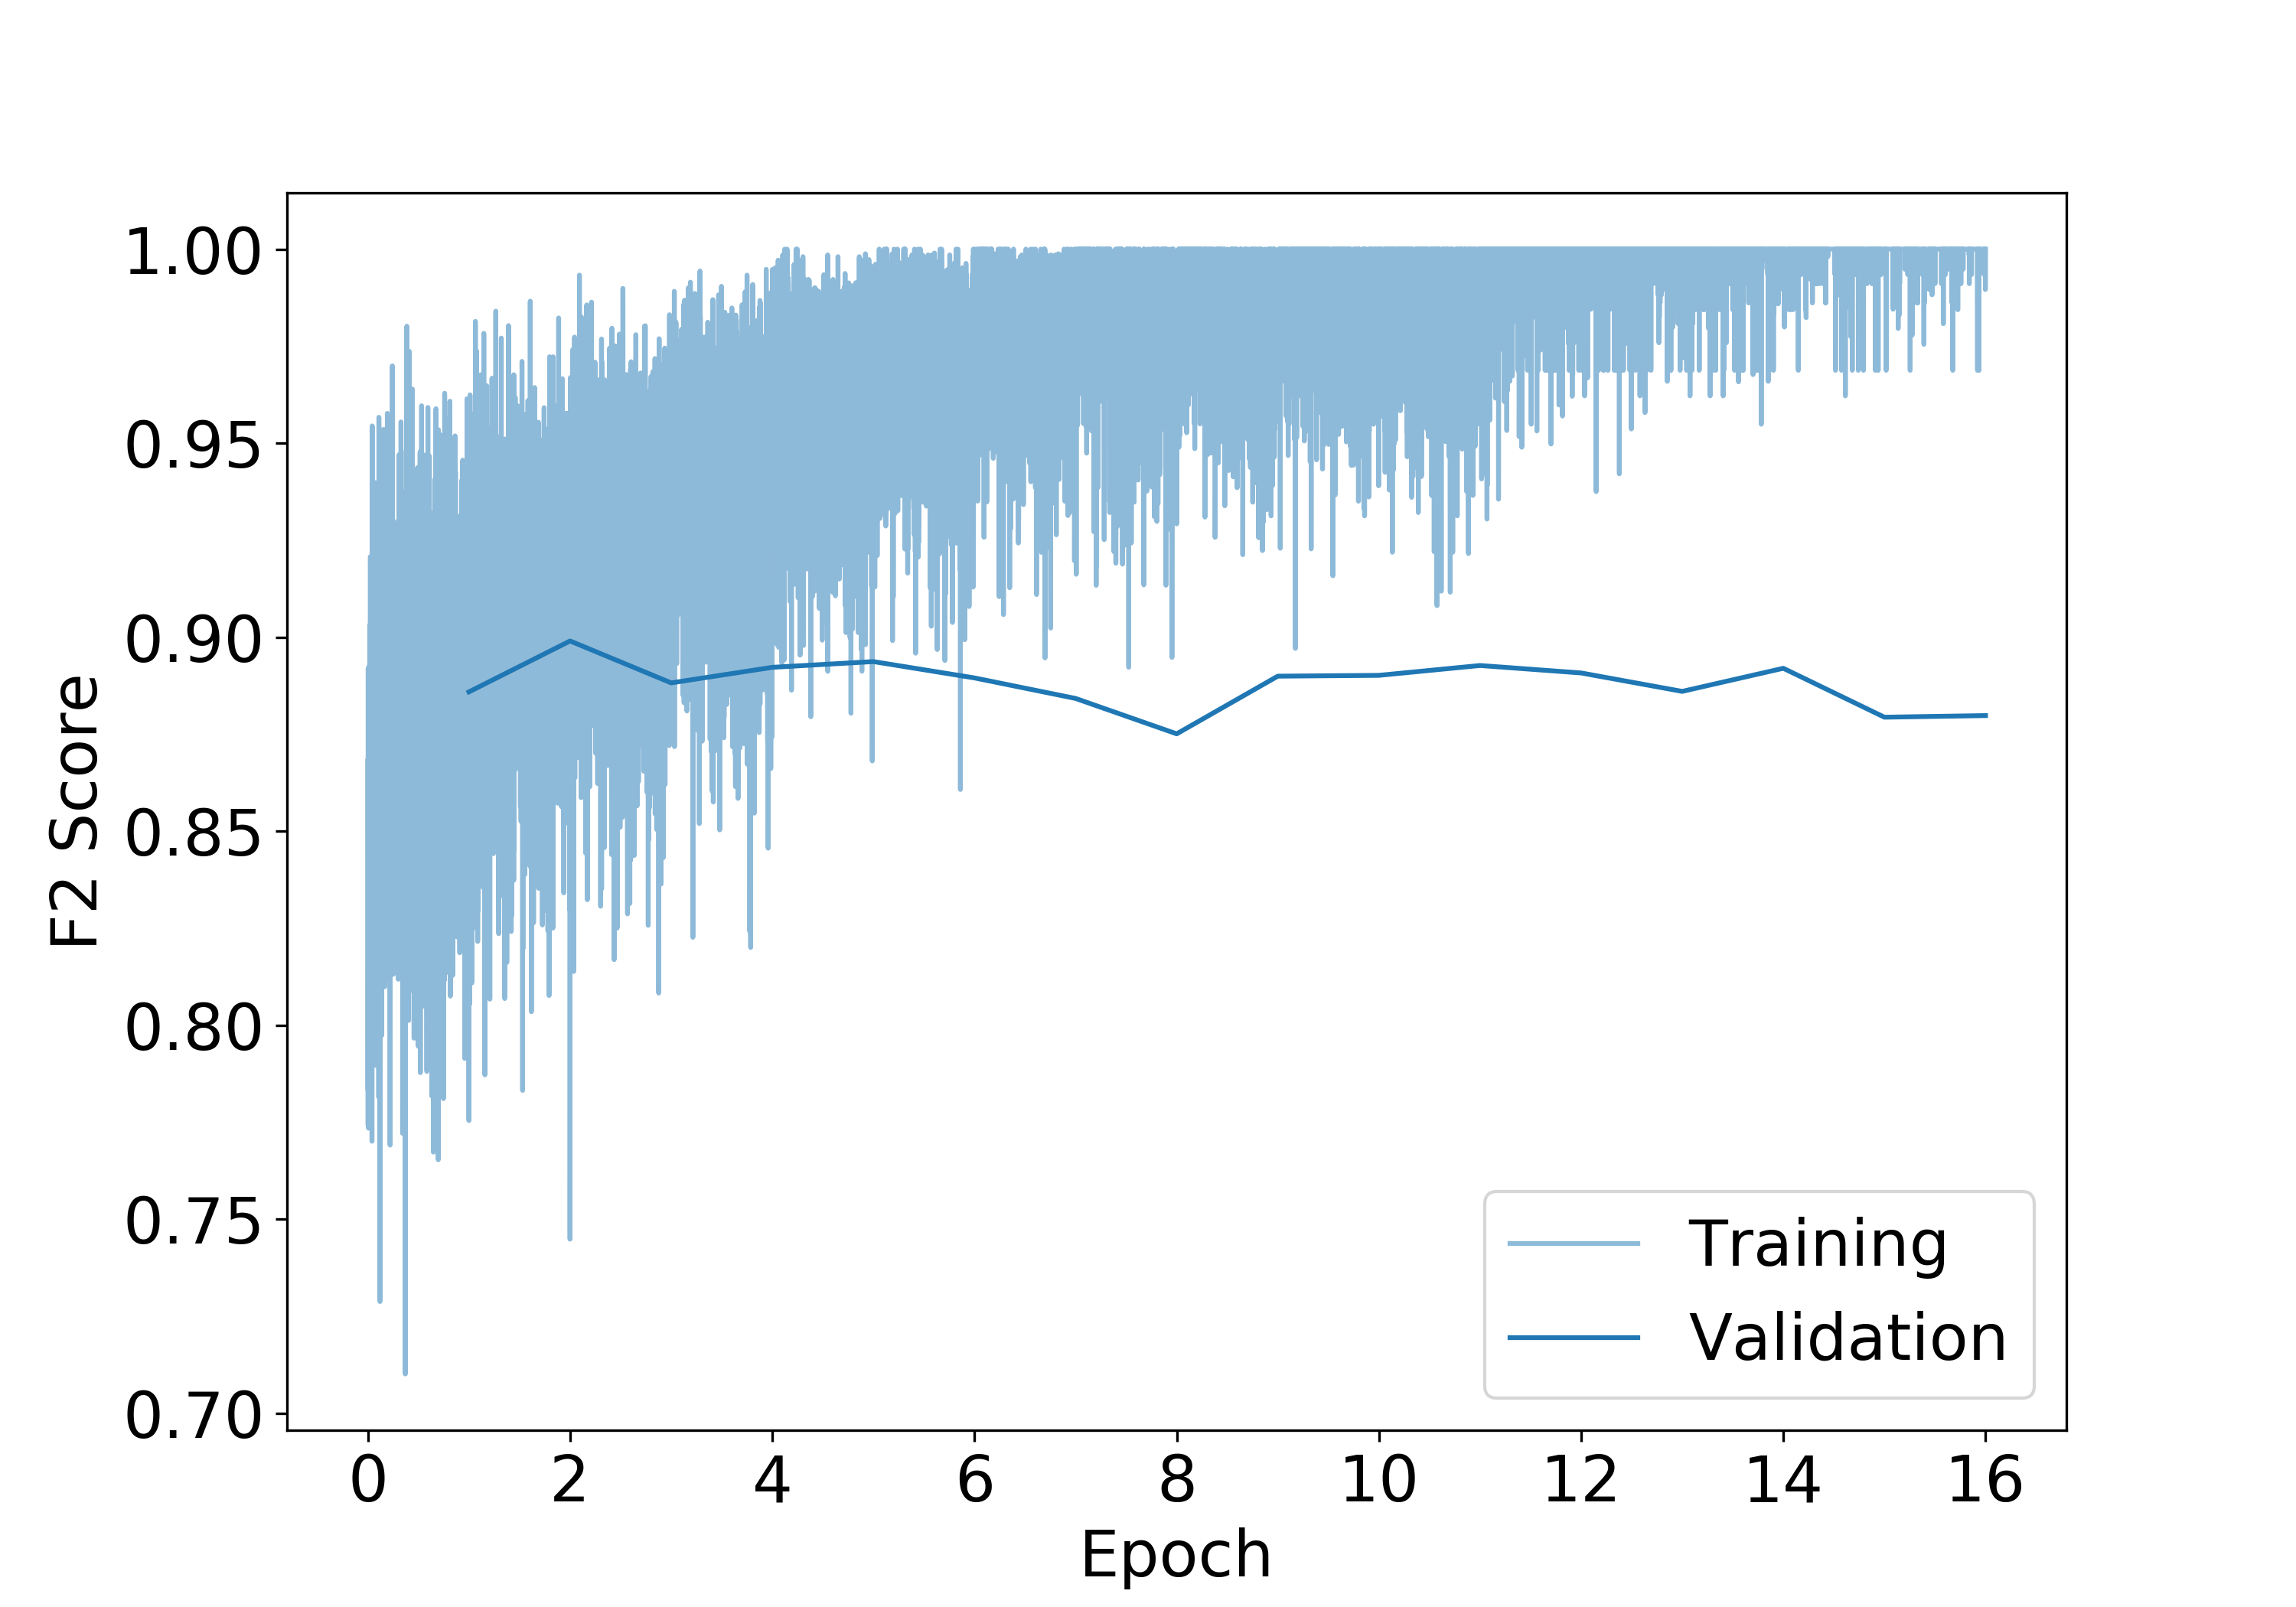
\includegraphics[width=\columnwidth]{fig/plot_validation_accuracy_resnet101_pretrained_tune.png}
    \caption{Pretrained ResNet101, training and validation accuracy during fine-tuning of all model weights}
    \label{fig:plot_validation_accuracy_resnet101_pretrained_tune}
\end{figure}

\subsection*{Pretrained Triple ResNet18}

Another strategy we pursued for improving on our initial results was to leverage the multiple data sets available for training in this challenge (data from .jpg and .tif versions of the files) and create an ensemble of separately-trained ResNets. To do so, we individually trained three ResNet-18's on different data sets and combined their scores to make our predictions. One ResNet was trained on the RGB channels ('rgb'), another on the near-infrared channel mapped to 3 color bands ('inf'), and a third on grayscale, $\nabla_x$, and $\nabla_y$ ('grad'). We elected to train a separate model for each, rather than combine all the channels into the input for a single model so that we could continue to work with pretrained ResNets rather than training from scratch.

Figure \ref{fig:plot_loss_triple_resnet18_tune} shows the loss during training for the three individual models. Note that loss is much higher for the 'inf' and 'grad' datasets than for 'rgb'. This is because the training labels were created by humans using the 'rgb' data and so the 'rgb' data corresponds more faithfully to the labels identified in the images. Figure \ref{fig:plot_validation_accuracy_triple_resnet18_tune} shows the accuracy for the three individual models during training. All three models do not overfit the training data. As expected, the accuracy is much higher for the 'rgb' model than the 'inf' and 'grad' models. 

As summarized in Table \ref{tab:summary}, the Triple ResNet18 model gives the strongest performance on the test set of any of our models: test F2 of 0.918. To achieve this, we maximize the F2 score by optimizing the weights used when combining the scores from the three models as described in the Methods section. We also optimize the cutoffs for the sigmoid function after combining the scores from the three models as described in the Methods section. Interestingly, the score of the combined model is higher than the score any of its individual components.

\begin{figure}
	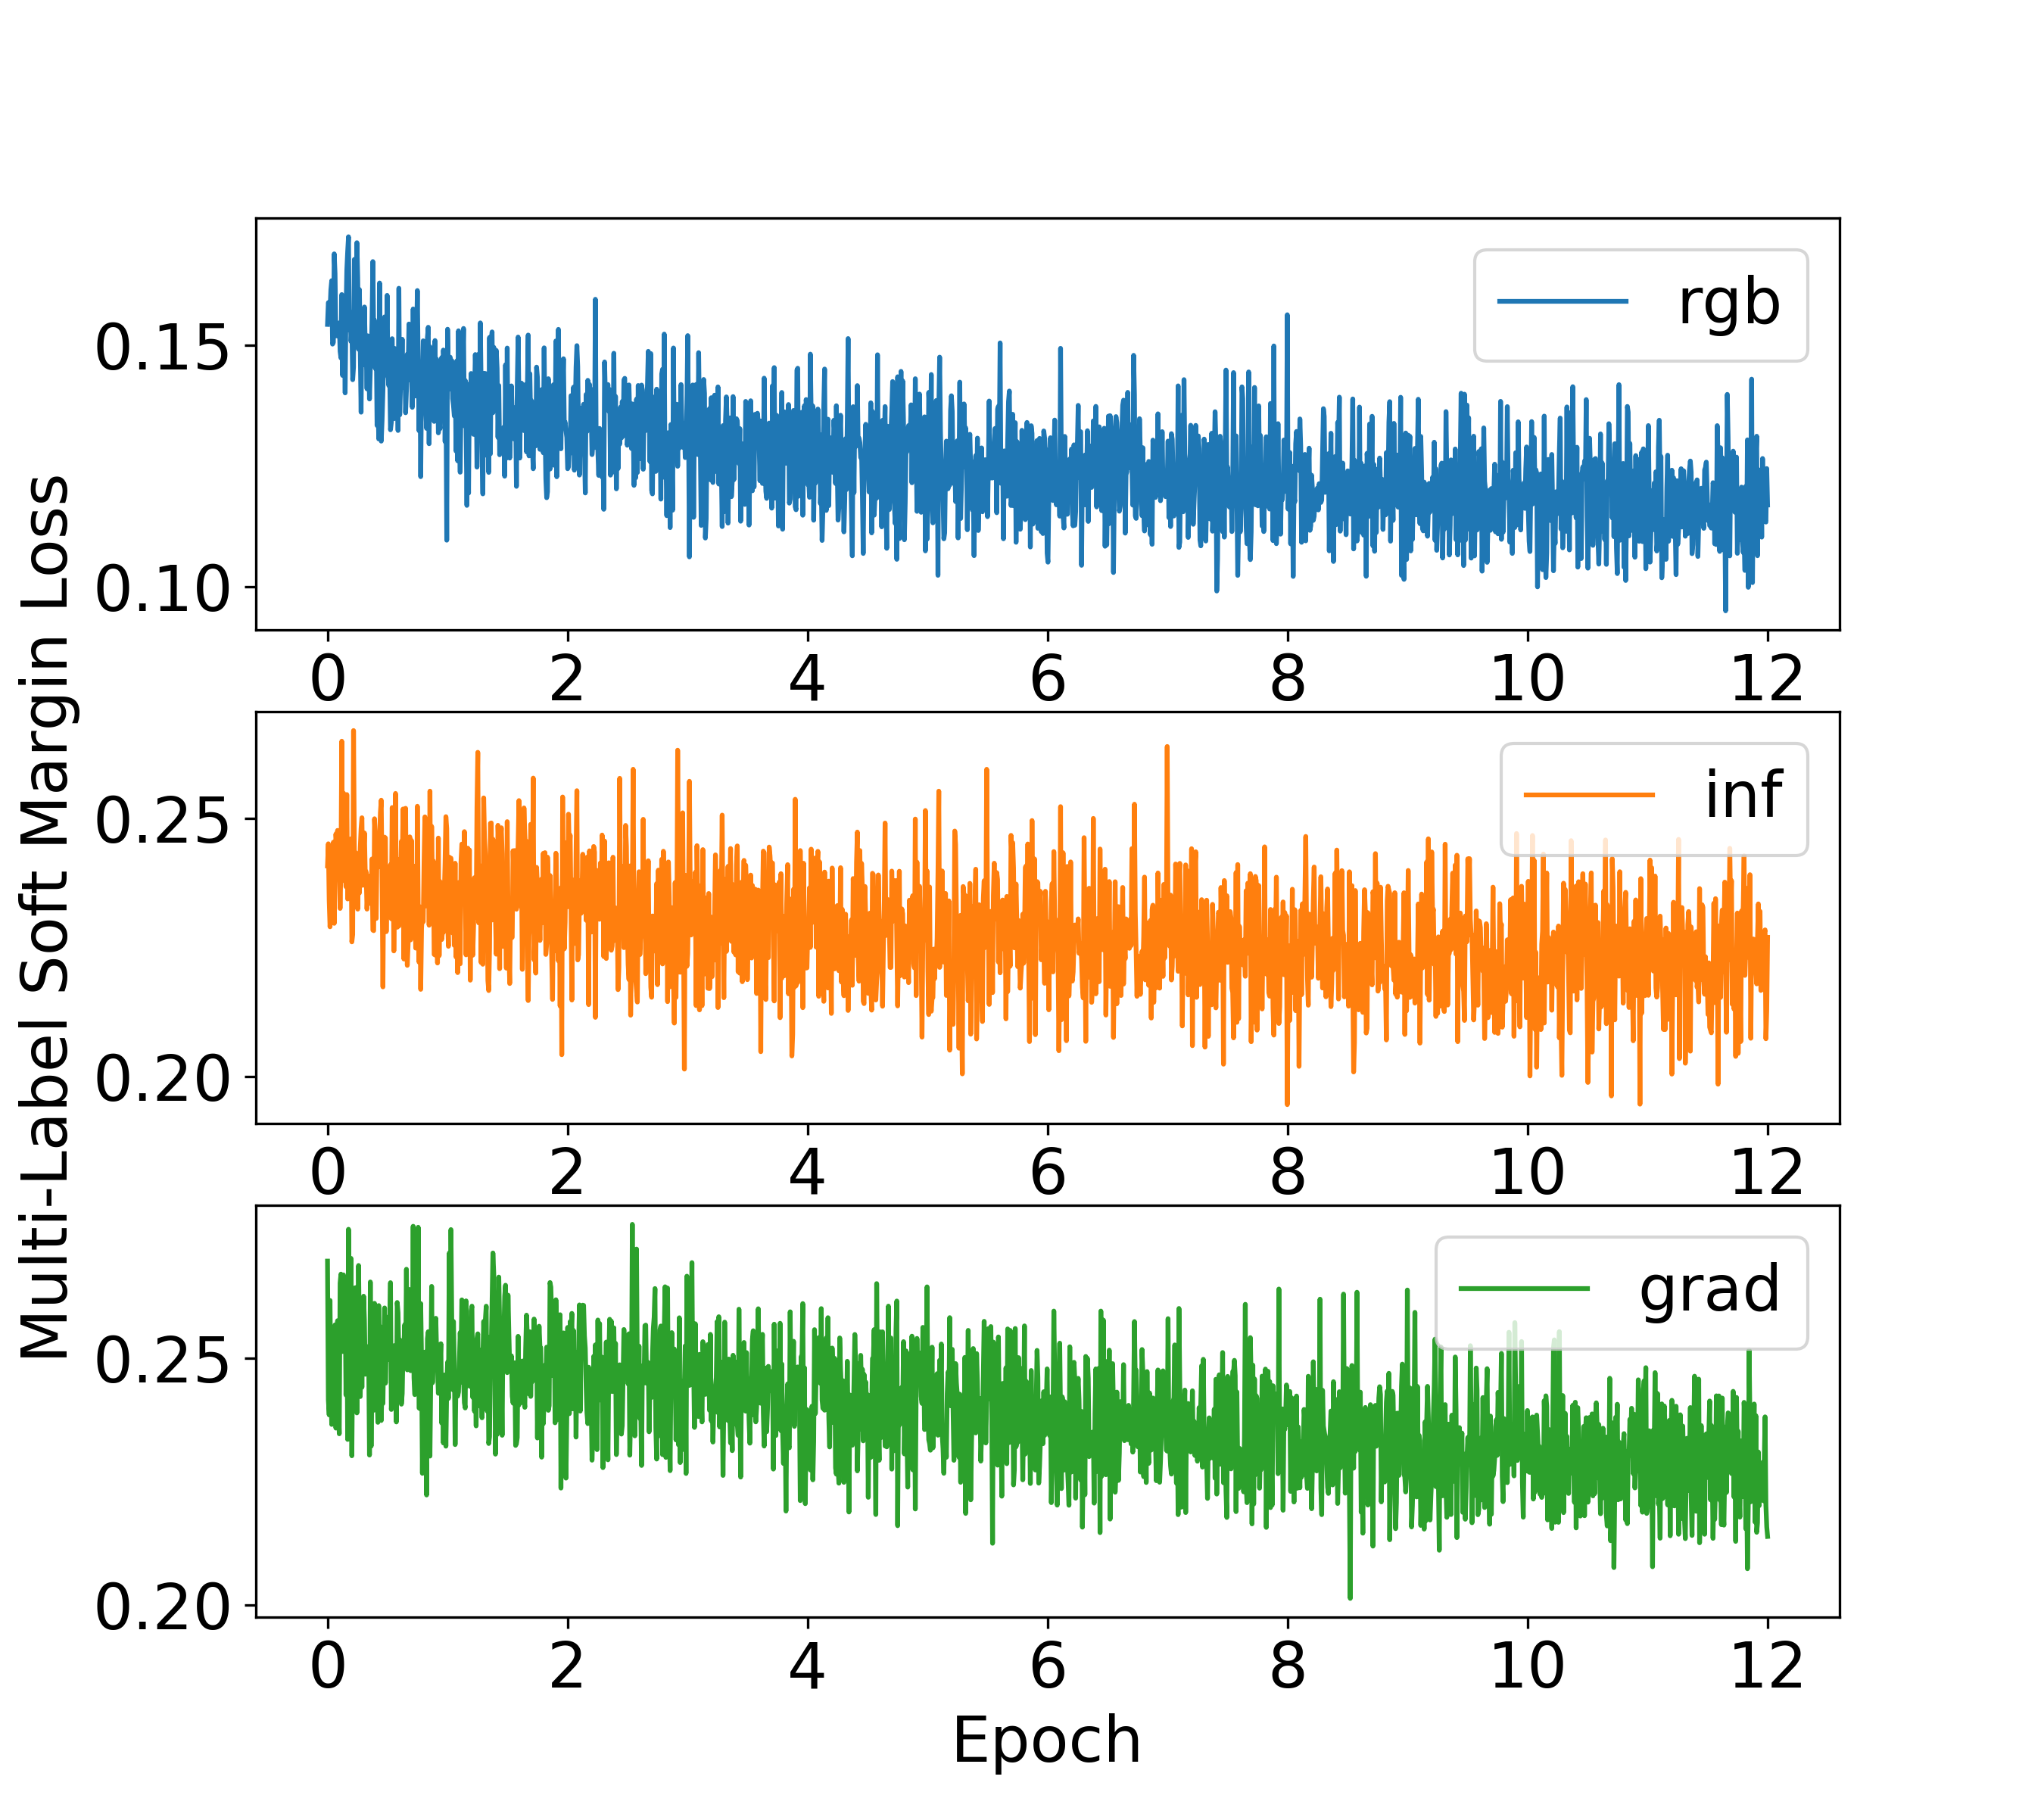
\includegraphics[width=\columnwidth]{fig/plot_loss_triple_resnet18_tune.png}
    \caption{Loss for the Triple ResNet18 individual models as a function of time.}
    \label{fig:plot_loss_triple_resnet18_tune}
\end{figure}

\begin{figure}
    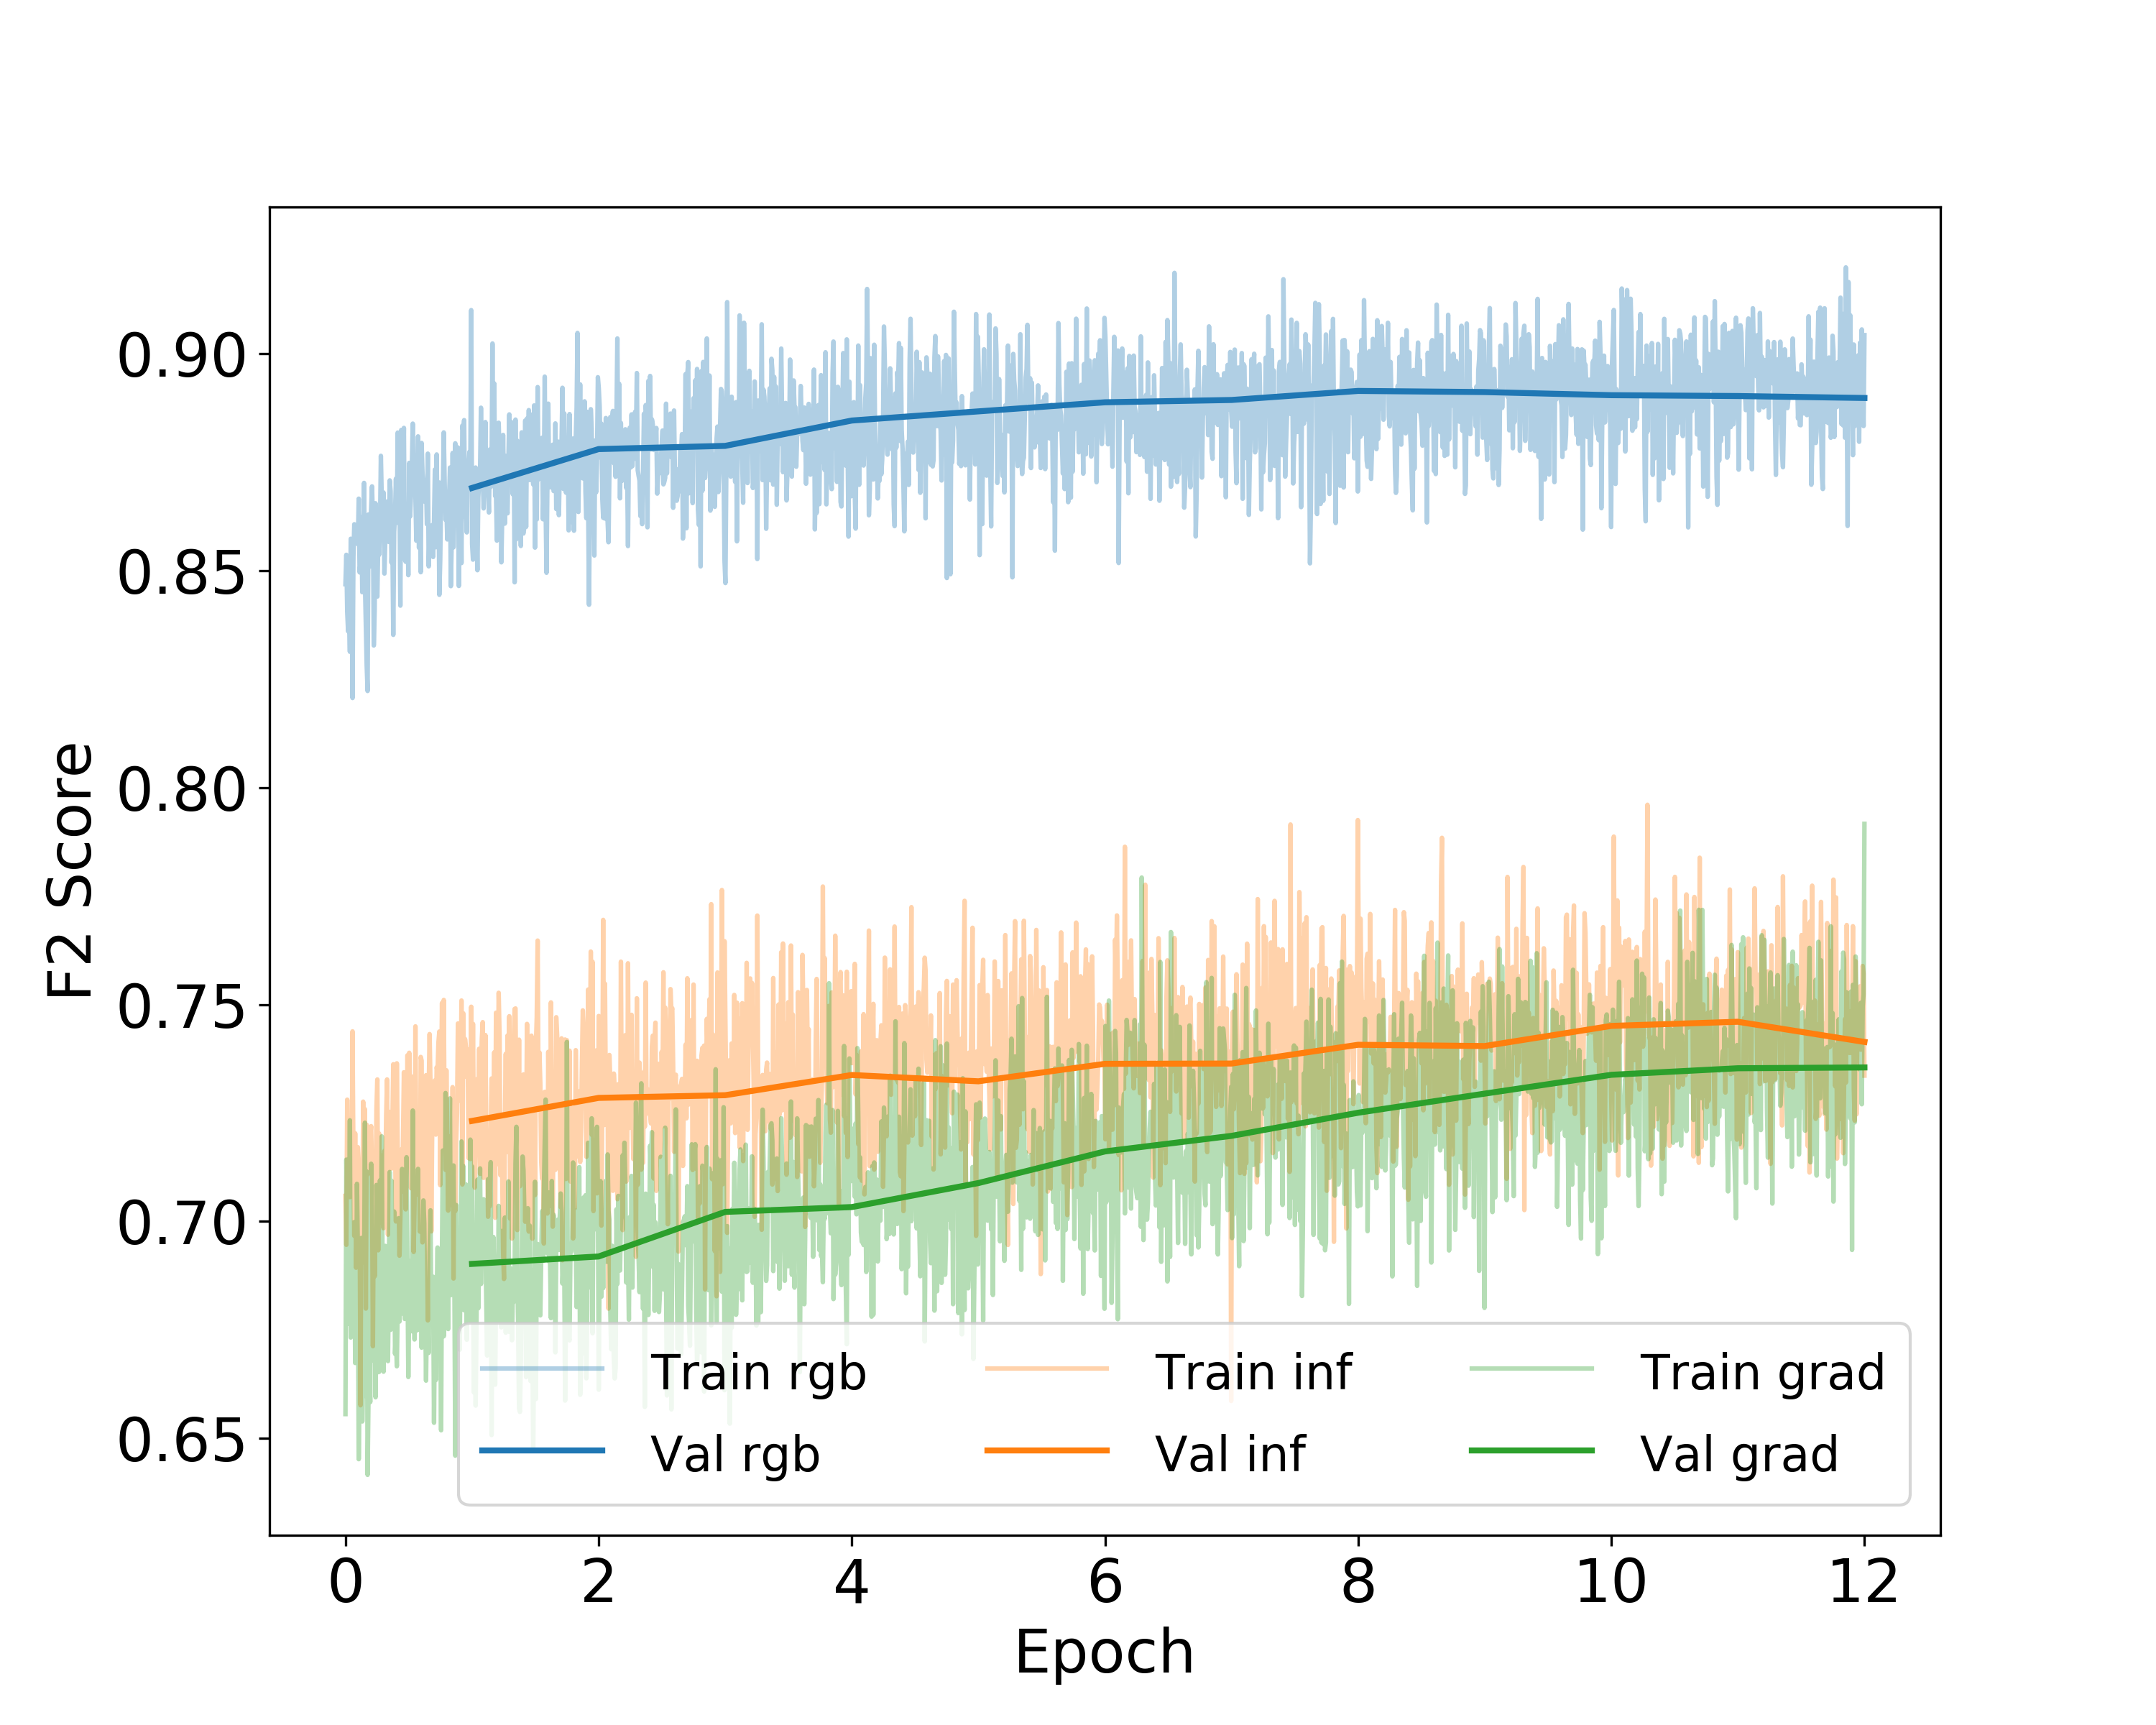
\includegraphics[width=\columnwidth]{fig/plot_validation_accuracy_triple_resnet18_tune.png}
    \caption{Accuracy (F2 score) results for the Triple ResNet18 individual models on the training set and the validation set as a function of epoch. The training accuracy was plotted at the end of each batch of data, and the validation accuracy was plotted at the end of each epoch.}
    \label{fig:plot_validation_accuracy_triple_resnet18_tune}
\end{figure}

\subsection*{ResNet18 from scratch}

\begin{figure}
	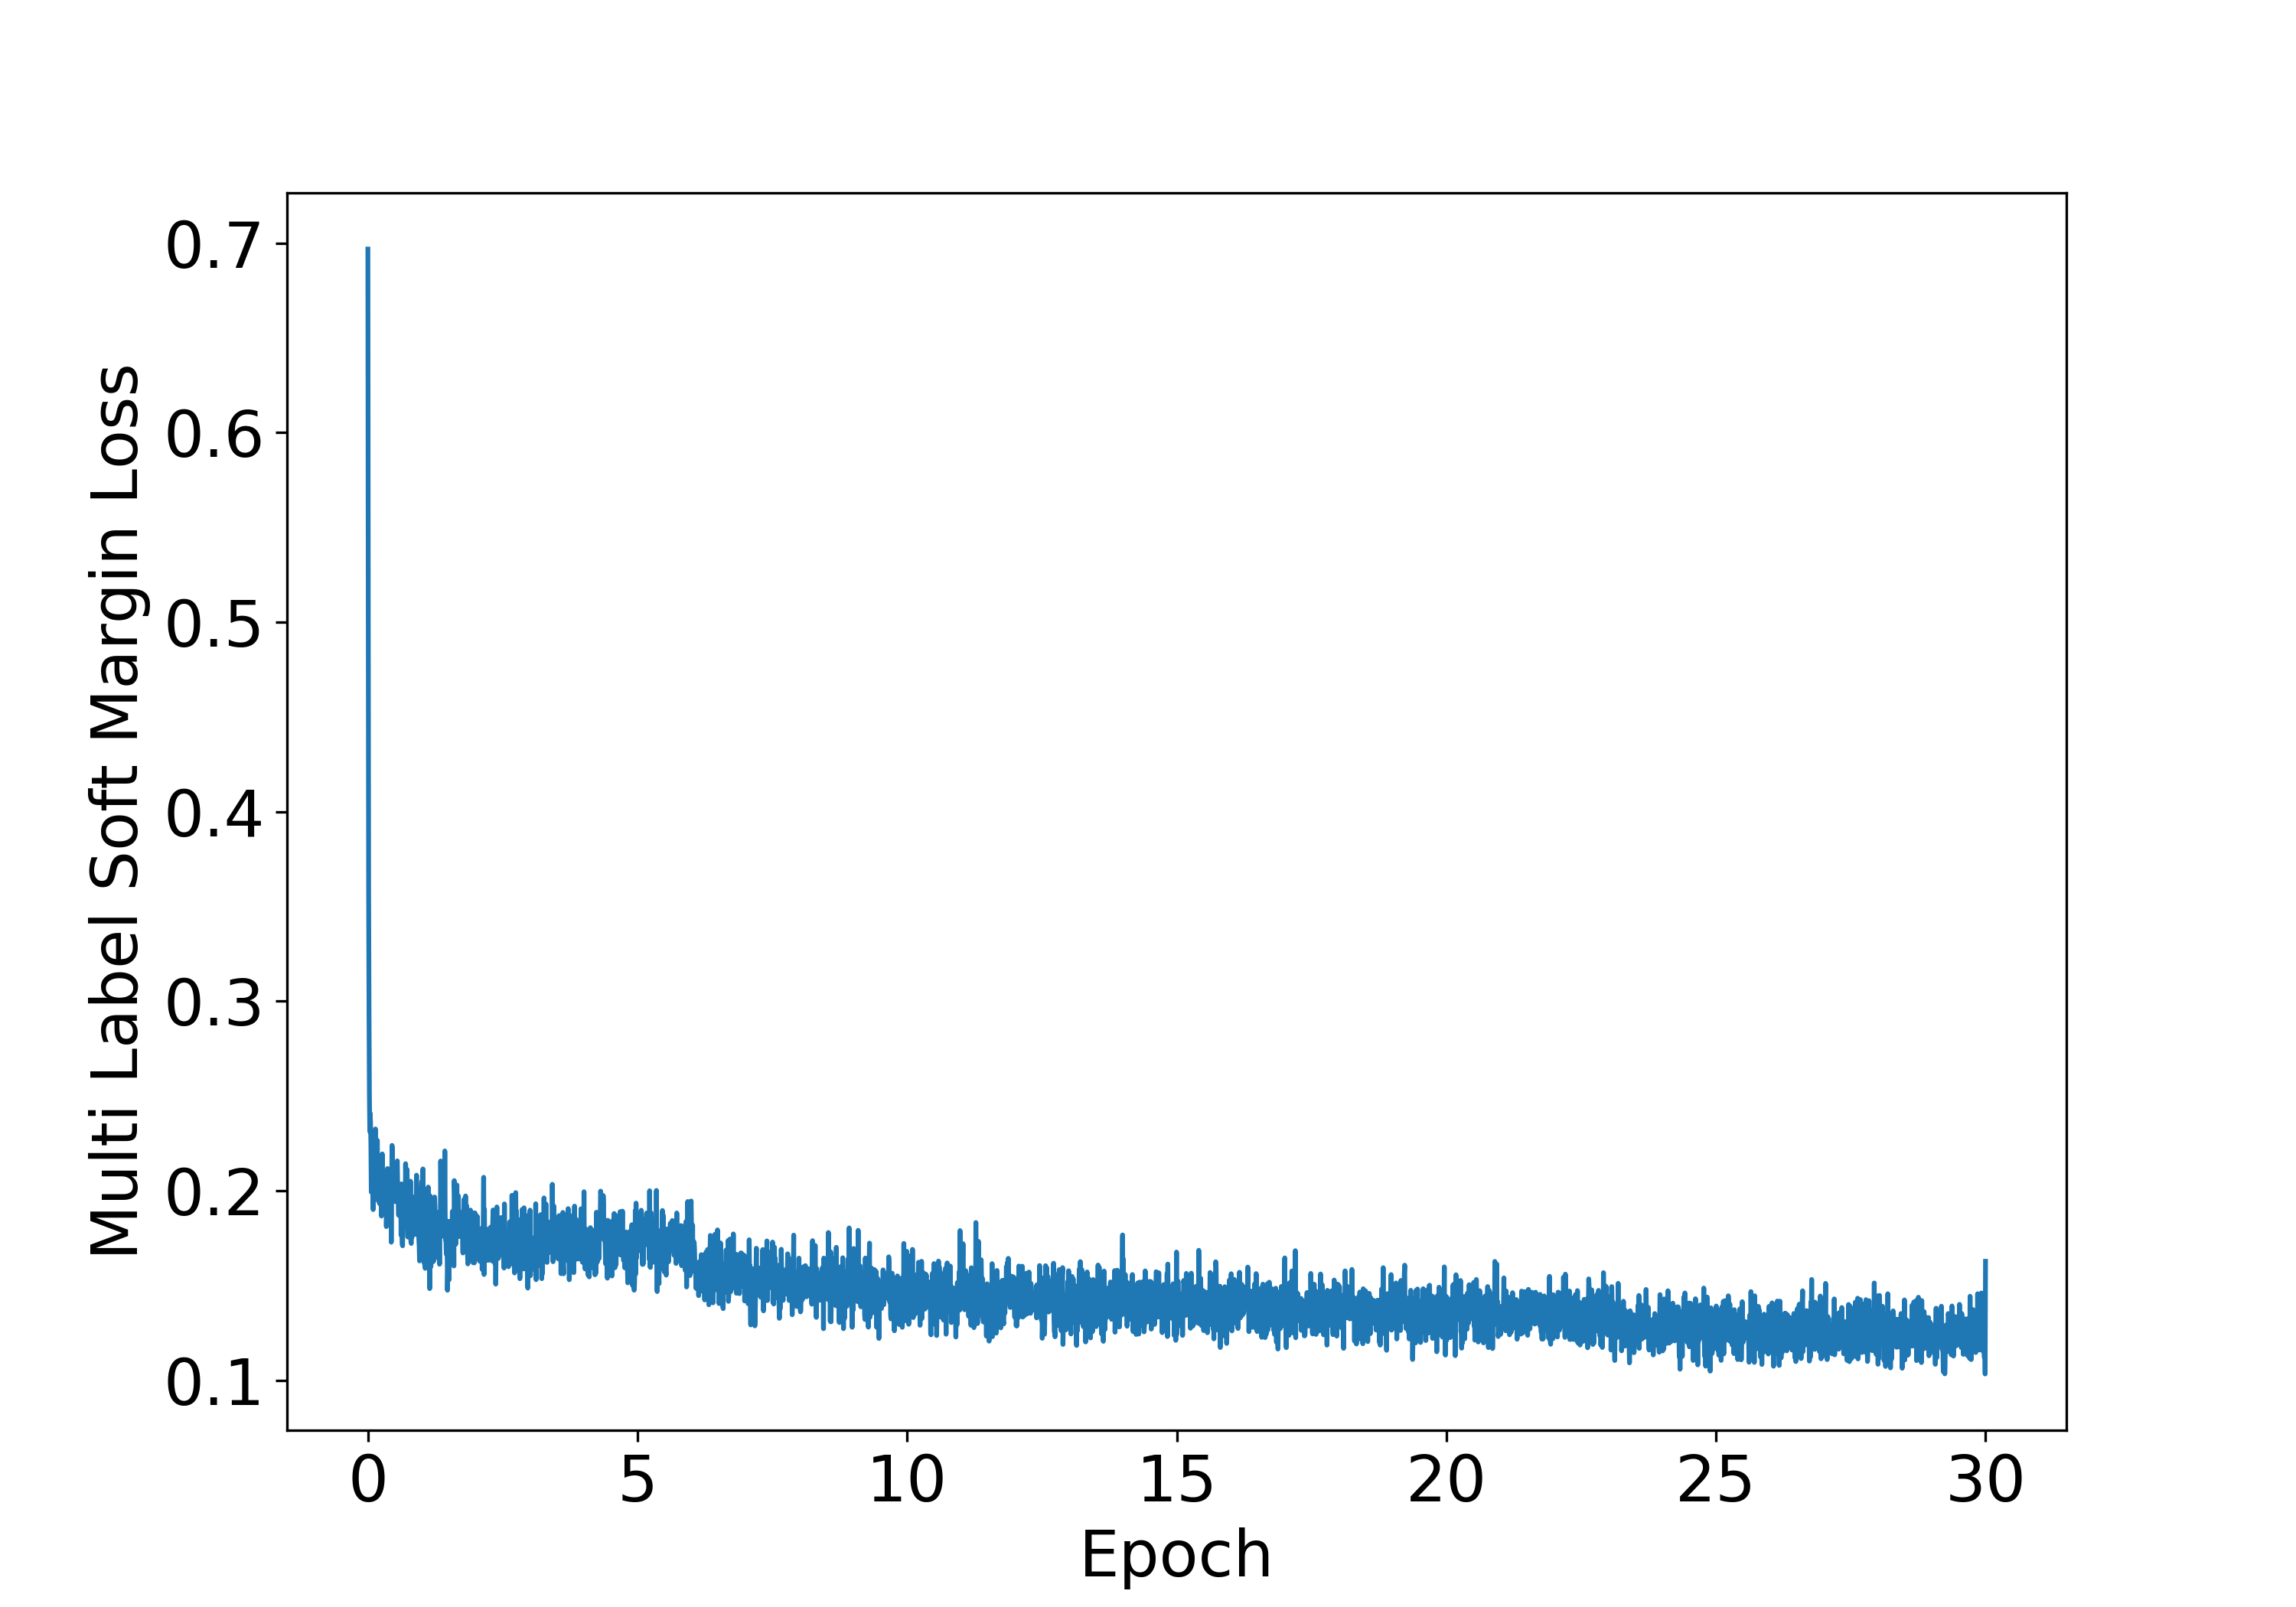
\includegraphics[width=\columnwidth]{fig/plot_loss_resnet18_rgb.png}
    \caption{ResNet18 from scratch, loss during training}
    \label{fig:plot_loss_resnet18_rgb}
\end{figure}

\begin{figure}[t]
    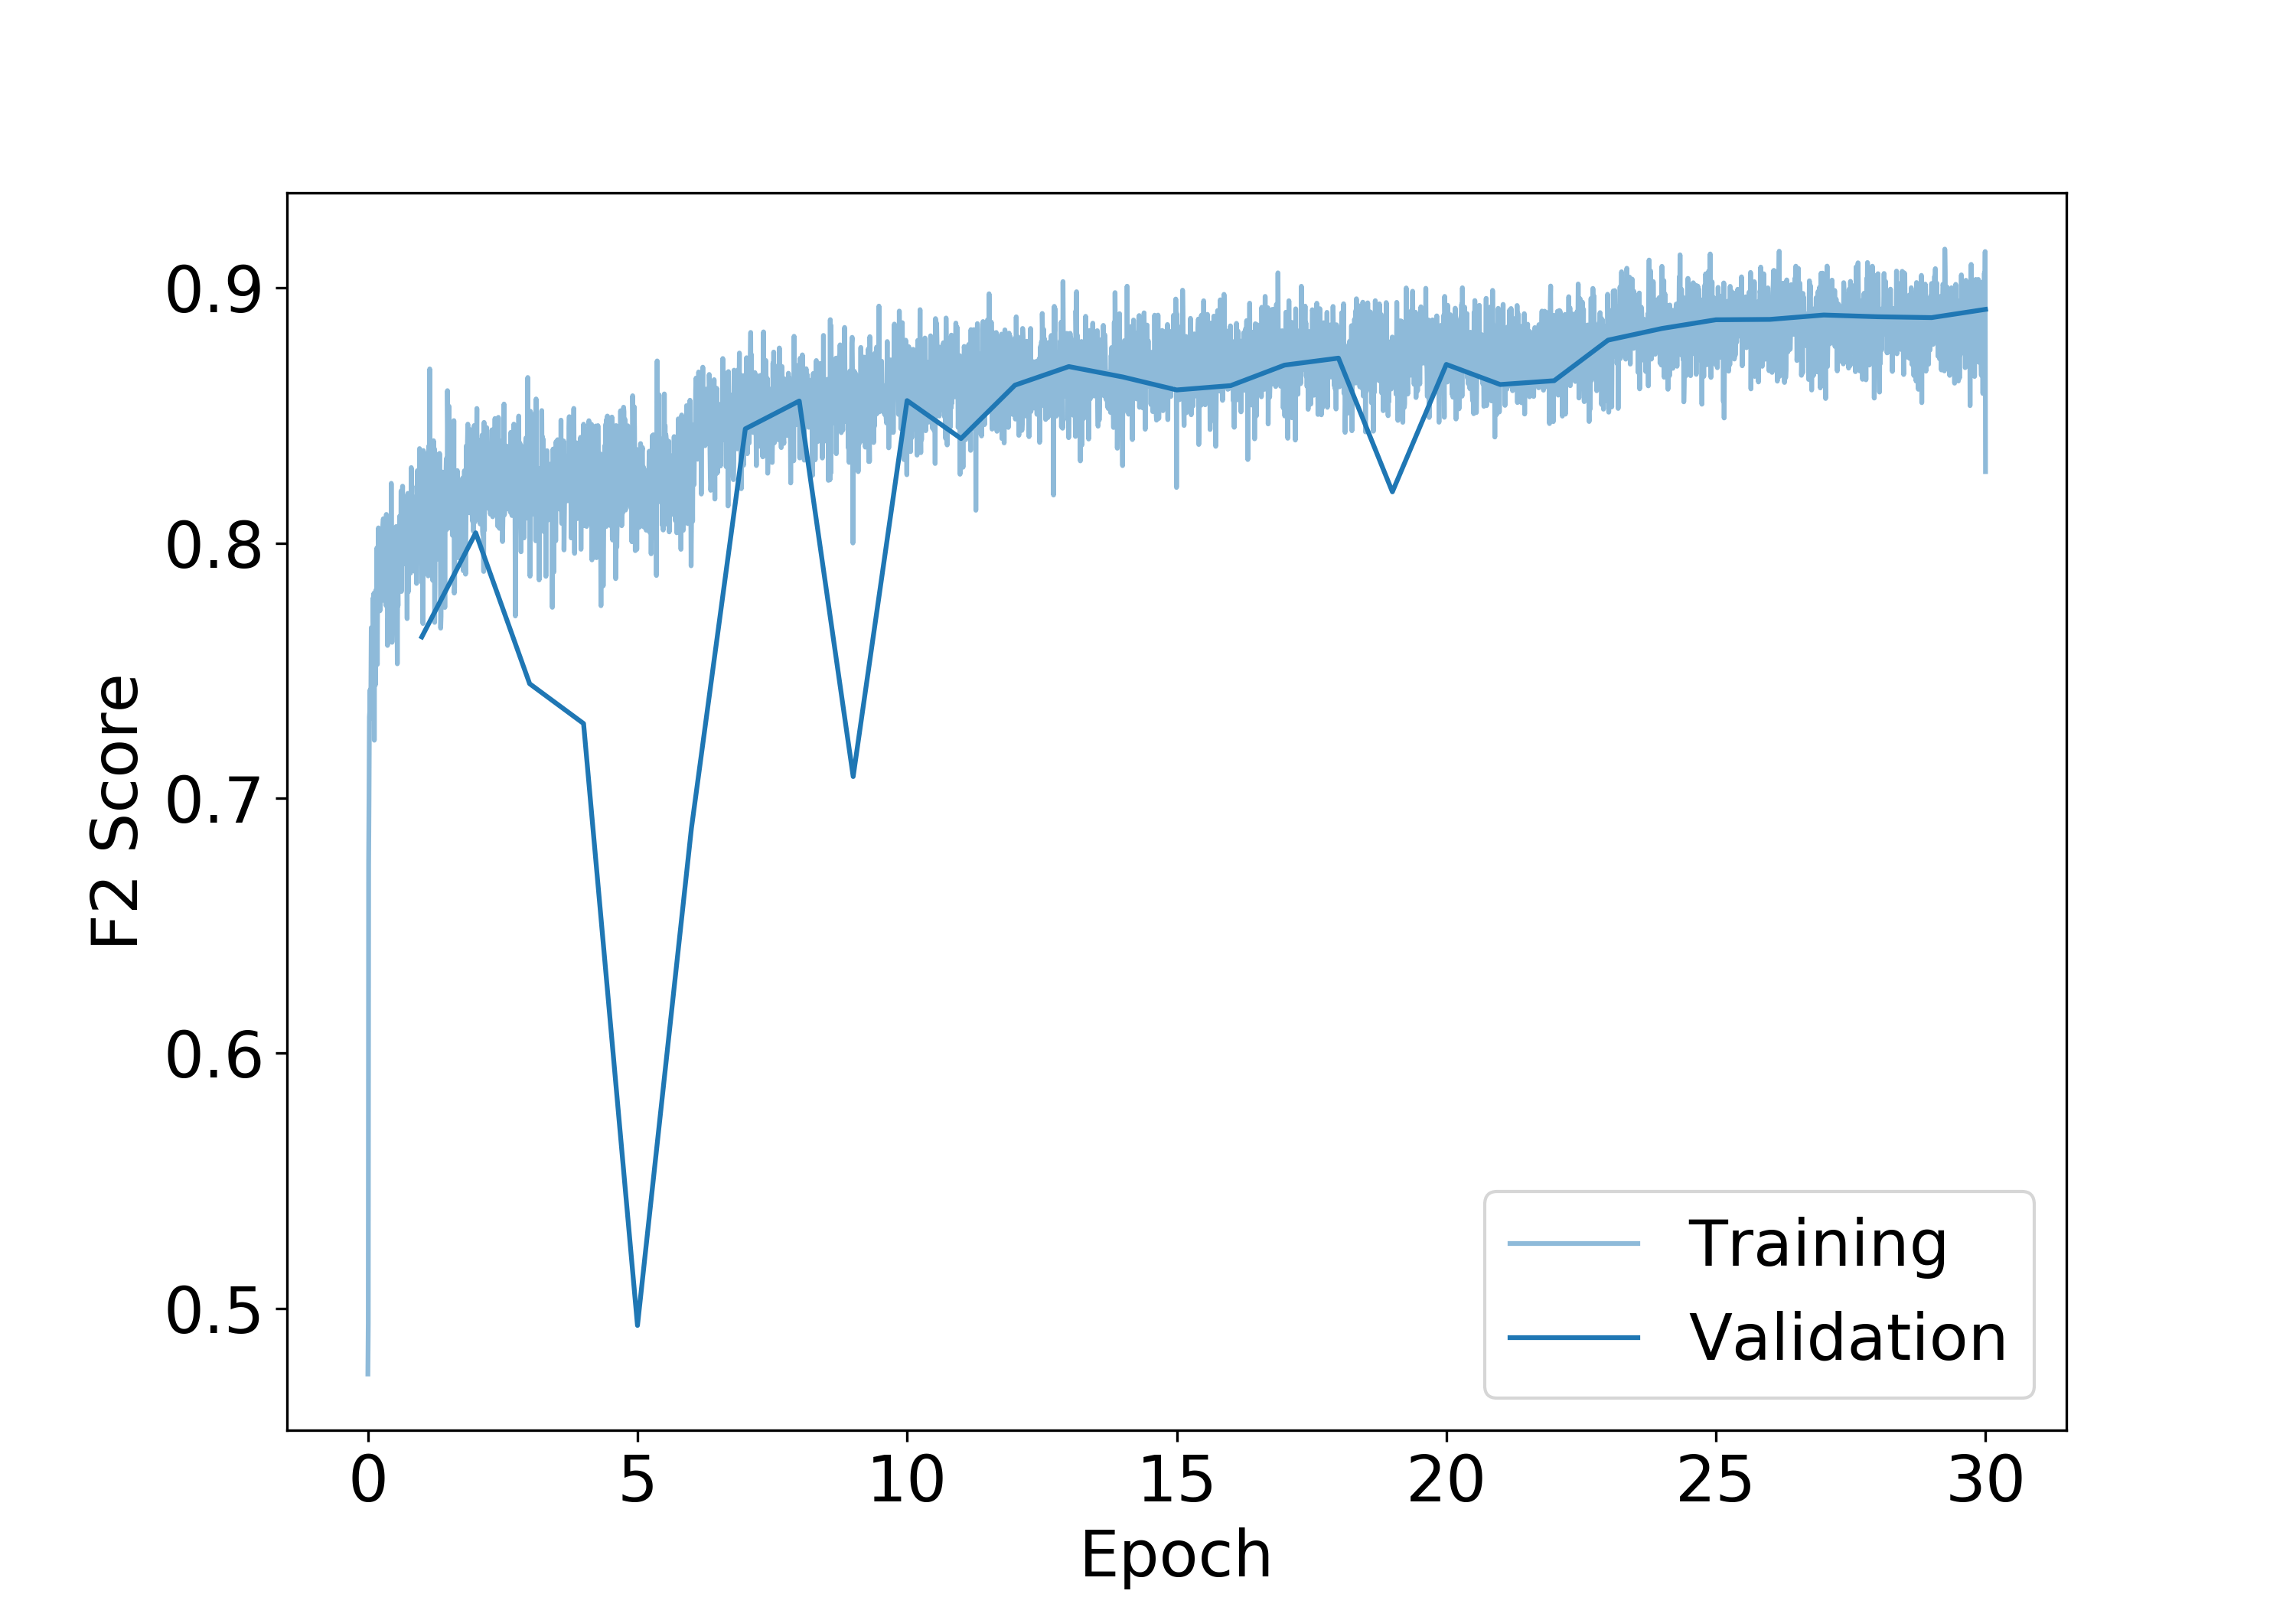
\includegraphics[width=\columnwidth]{fig/plot_validation_accuracy_resnet18_rgb.png}
    \caption{ResNet18 from scratch, accuracy (F2 score) results for the training and validation datasets}
    \label{fig:plot_validation_accuracy_resnet18_rgb}
\end{figure}

Having explored a variety of approaches using pretrained ResNets, and since some studies find that training from randomly initialized weights gives better results than fine-tuning pretrained models,\cite{fromscratch2} we next investigated the performance of a ResNet18 trained from randomly initialized weights. The ResNet was trained on the 'rgb' dataset for 30 epochs using a weight regularization of 1e-3 and a learning rate initialized at 1e-3, which adaptively decreases when loss stagnates. Figure \ref{fig:plot_loss_resnet18_rgb} shows the loss during training for this model. The role of the adaptive learning rate can be seen in the sharp jumps down in loss that occur at the end of stagnant periods (for example, at the end of epoch 6). Figure \ref{fig:plot_validation_accuracy_resnet18_rgb} shows the evolution of the F2 scores on the training and validation data. The model does not overfit the training data, at the end of 30 epochs the validation accuracy is still roughly the same as the training accuracy. There are several instances where the validation accuracy sharply decreases and then recovers (for example, at epoch 5). These features do not appear when fine-tuning the pretrained models. This is likely because when the pretrained models are fine-tuned, they are already near a local minimum in the new loss landscape. However, the models trained from randomly initialized weights must traverse the high-dimensional loss landscape from a random point to the best minimum that the optimizer can find. Along that path, there are some points that have very high generalization error, but in the end, the model converges to a minimum with low generalization error.


%------------------------------------------------------------------------
\section{Conclusions and Future Work}

In this project, we trained convolutional neural networks to perform multilabel classification of land usage from satellite images of the Amazon Rainforest. We have trained a variety of networks including custom designed convolutional architectures, ResNets, and GoogleNets. Our highest performing model to date is an averaging of three ResNet18s, trained using transfer learning. This model achieves an F2 score of 0.918 on the test set.
In our work so far, we largely focused on fine-tuning pretrained ResNets. In our future work, we intend to explore training the ResNet models from scratch. We intend to use new input data combining all seven of the unique channels available between the .jpg and .tif datasets. This should improve results as the network can learn weights to combine all of the available input data, whereas in our current highest scoring model the different bands of data are grouped into sets of three and their predictions are only combined after training. We also want to further explore model ensembles, which will help the overall model find a global minimum by averaging several models that are converged to nearby local minima in the loss landscape. The leaders of the Kaggle competition have an F2 score only about 0.015 than our current best model, so we hope that the proposed future work will be able to bring our model closer to the state-of-the-art.


%------------------------------------------------------------------------

\clearpage
{\small
\bibliographystyle{ieee}
\bibliography{references}
}

\end{document}
